\chapter{Projekt i implementacja środowiska badawczego}
\label{chap:implementacja-systemu}
W niniejszym rozdziale opisana została implementacja kluczowych funkcjonalności systemu. W ramach opisu, przedstawiono elementy kodu źródłowego programu wraz z ich wyjaśnieniami.

W pierwszych dwóch podrozdziałach, omówiona została zasada działania interfejsu programowania aplikacji. Ukazano w nich między innymi pełny przepływ wykonywanych operacji w momencie wywołania punktu końcowego API.

W podrozdziale trzecim, przeanalizowano koncepcję mechanizmu zarządzania stanem aplikacji oraz aktualizacji treści bez przeładowywania strony. Koncepcje ta, są określone w sposób identyczny, zarówno dla aplikacji mobilnej jak i webowej.

Następne części odnoszą się kolejno do funkcjonalności aplikacji webowej oraz mobilnej. Niektóre spośród tych funkcjonalności są wspólne dla obu aplikacji, dlatego też przedstawione zostaną tylko w kontekście danego elementu systemu.

Ostatni z podrozdziałów stanowi o implementacji graficznego interfejsu użytkownika. Poza kodem źródłowym widoków systemu, zaprezentowane są w nim również ilustracje przedstawiające gotowy interfejs.

\section{Interfejs programowania aplikacji (API)}
\label{sec:api-implementacja}
Zgodnie z informacjami wprowadzonymi w podrozdziale \ref{subsec:architektura-aplikacji}, interfejs programowania aplikacji API, zbudowany został w oparciu o architekturę trójwarstwową. W strukturze tej, po wysłaniu żądania z wykorzystaniem protokołu hipertekstowego, zostaje ono obsłużone przez określoną metodę klasy kontrolera. Metoda ta, w celu ustalenia odpowiedzi na żądanie klienta, komunikować się musi z klasami niższych warstw modelu, określanymi jako serwisy.

Wewnątrz klas serwisów, wykonywane są operacje z dziedziny logiki biznesowej. W operacjach tych, wymagane są najczęściej dane, które metoda serwisu mogłaby przetwarzać. Aby te dane uzyskać, podobnie jak metody kontrolerów, tak i metody warstwy logiki biznesowej odwoływać się muszą do klas warstw niższych. Takie klasy, w kontekście zrealizowanego oprogramowania nazywane są repozytoriami.

Mechanizm odwołań do klas warstw niższych w celu pozyskiwania niezbędnych do przetwarzania informacji umożliwia proste rozdzielenie odpowiedzialności w ramach realizowanych funkcji. Ponadto, pozwala on na implementację elastycznego mechanizmu obsługi błędów oraz łatwiejsze wykrywanie potencjalnych problemów.

Na listingach \ref{lst:endpoint-forward-worker}, \ref{lst:service-forward-worker} i \ref{lst:repository-forward-worker}, określone zostały fragmenty kodu źródłowego metod, dla klas z poszczególnych warstw architektury aplikacji. Wszystkie z listingów są ze sobą powiązanie, ponieważ stanowią fragmenty realizacji odpowiedzi na to samo żądanie klienta.

Poniżej przedstawiono sposób obsługi żądania typu POST dla punktu końcowego \texttt{/api/documents/forwards/worker}, odpowiedzialnego za realizację przekazania dokumentu pracownikowi.

Po wysłaniu żądania HTTP, dla określonego w akapicie powyżej adresu punktu końcowego, wykonany zostanie kod metody z listingu \ref{lst:endpoint-forward-worker}. W pierwszym wierszu tej metody, określona została adnotacja \textit{(ang. Data Annotation)} dotycząca typu obsługiwanego żądania, oraz fragmentu jego adresu. Metoda jest asynchroniczna (tj. uruchamiana jest jako oddzielny wątek programu i cechuje się sekwencyjnością realizacji operacji niezależnie od czasu ich trwania).

Funkcja punktu końcowego przyjmuje jako argument zasób \textit{(ang. Resource)}. Element ten, definiuje parametry związane z nadawcą, odbiorcą oraz przekazywanym dokumentem. Wartość zasobu, można przekazać metodzie endpoint'u poprzez zdefiniowanie ciała żądania HTTP \textit{(ang. HTTP Body)}. W przypadku realizowanego API, ciało żądania posiada formę obiektu JSON.

Na początku metody, przekazany argument (zasób) poddawany jest walidacji. Walidacja może przebiec niepomyślnie w sytuacji, w której elementy obiektu JSON będą posiadały niepoprawne typy danych, lub wymagane wartości nie zostaną w nim zdefiniowane. Po pomyślnym przejściu procedury walidacji, obiekt zasobu oraz zagnieżdżony w nim zasób dokumentu odwzorowywane są na obiekty klas modelu danych. Pozwala to, na przekazanie ich jako parametry do metody klasy warstwy niższej - serwisu.

Po uzyskaniu wartości zwróconej przez serwis, w metodzie kontrolera sprawdzana jest jej poprawność. W zależności od wyniku tego sprawdzenia, wysyłana jest odpowiedź HTTP sygnalizująca błąd wykonywanej operacji lub jej powodzenie. Zgodnie ze standardem REST \textit{(ang. Representational State Transfer)}, wykorzystywanym przez system jako zbiór zasad dotyczących działania API, w przypadku poprawności metody punktu końcowego dla typu operacji POST, zwracana jest pusta zawartość \textit{(ang. No Content)}.

\begin{lstlisting}[label=lst:endpoint-forward-worker,caption=Kod metody punktu końcowego przekazywania dokumentów pracownikowi, captionpos=b,basicstyle=\footnotesize\ttfamily,style=sharpcstyle,language={[Sharp]C}]
[HttpPost("worker")]
public async Task<IActionResult> ForwardToWorkerAsync([FromBody] ForwardToWorkerResource res) {
	
	if (!ModelState.IsValid) {
		return BadRequest(ModelState.GetModelStateErrorMessagesInfo());
	}
	
	var documentsForward = mapper.Map<ForwardToWorkerResource,DocumentsForward>(res);
	var document = mapper.Map<ForwardDocumentResource,ForwardDocument>(res.Document);
	var result = await documentsForwardService.ForwardToWorker(documentsForward, document);
	
	if (!result.Success)
		return BadRequest(result.Message);
		
	return NoContent();
}
\end{lstlisting}

W linii dziewiątej listingu \ref{lst:endpoint-forward-worker} metoda kontrolera API wywołuje metodę serwisu. Linia ta, jest kluczowym fragmentem kodu źródłowego punktu końcowego, ponieważ właśnie w metodzie serwisu wykonywane są operacje związane z faktycznym przekazaniem dokumentu pracownikowi. Omawiana w następnym akapicie funkcja serwisu przedstawiona jest na listingu \ref{lst:service-forward-worker}.

Do metody przekazania dokumentu, dostarczane są dwa argumenty. Pierwszym z nich jest obiekt zasobu, natomiast drugi stanowi zasób faktury. Elementy te, zgodnie z informacjami przedstawionymi uprzednio, zostały wcześniej przekształcone z obiektowej notacji JavaScript na klasy modelu danych.

Początkowo, weryfikowane jest istnienie dokumentu w systemie na podstawie jego identyfikatora. Jeżeli dany rachunek nie został znaleziony, jest on generowany w oparciu o dane zawarte w zasobie dokumentu.

Następnie, weryfikowane są informacje związane z nadawcą oraz adresatem faktury. Dla prawidłowego przekazania dokumentu, dane obu pracowników (tj. ich identyfikatory) muszą być prawidłowe. W sytuacji wykrycia nieprawidłowości dla danych o pracownikach, metoda serwisu zwraca sterowanie do metody kontrolera, przekazując nowy obiekt odpowiedzi \textit{(ang. Response)}. Gdy w obiekcie tym, przypisana zostaje właściwość wiadomości błędu \textit{(ang. Message)}, logiczny atrybut powodzenia wykonania funkcji \textit{(ang. Success)} przyjmuje wartość \texttt{false}. Pozwala to, na określenie poprawności realizacji zadania serwisu wewnątrz metody kontrolera.

Kolejno, pobierane są wszystkie przekazania przypisane do dokumentu. Jeżeli ich liczba, jest większa od zera, należy sprawdzić, czy osoba chcąca przekazać dokument, aktualnie znajduje się w jego posiadaniu. W tym celu, uzyskiwany zostaje ostatni element listy przekazań. Aby zweryfikować przynależność dokumentu do pracownika, identyfikator odbiorcy w ostatnim z przekazań musi być zgodny z numerem pracownika stanowiącego nadawcę dla nowego przekazania. W przeciwnym razie, generowany jest obiekt odpowiedzi i przekazywane zostaje sterowanie do metody kontrolera.

W ostatnim fragmencie kodu źródłowego funkcji serwisu, definiowany jest nowy obiekt przekazania dokumentu. Po jego utworzeniu, wywoływana zostaje metoda klasy repozytorium zapisująca przekazanie do kontekstu bazy danych. Aby zmiana danych w obrębie kontekstu, odwzorowana została w bazie danych wykonana musi zostać metoda \texttt{CommitTransactionAsync} dla instancji klasy \texttt{UnitOfWork}. Klasa ta, jest implementacją wzorca projektowego \textit{Jednostka pracy}, opisanego w rozdziale \ref{subsec:architektura-aplikacji}.

Instrukcją kończącą metodę serwisu jest zwrócenie nowego obiektu odpowiedzi. W tym przypadku, obiekt ten zamiast tekstem wiadomości błędu, jest inicjalizowany strukturą przekazania dokumentu. Dzięki temu, atrybut poprawności wykonania metody przyjmuje wartość true.

\begin{lstlisting}[label=lst:service-forward-worker,caption=Kod metody serwisu przekazywania dokumentów pracownikowi, captionpos=b,basicstyle=\footnotesize\ttfamily,style=sharpcstyle,language={[Sharp]C}]
public async Task<Response<DocumentsForward>> ForwardToWorker(DocumentsForward forward, ForwardDocument document) {		
			
	var existingDocument = await documentService.GetDocumentAsync(document.Id);
	Document documentToForward = null;
	if (!existingDocument.Success) {
			var result = await documentService.SaveAsync(document);
								
			if (!result.Success) {
					return new Response<DocumentsForward>("Błąd zapisu dokumentu:{...}");
			}
			documentToForward = result.Type;
	}
	else {
			documentToForward = existingDocument.Type;
	}

	var existingRemitter = await workerService.GetWorkerAsync(forward.RemitterId);
	var existingRecipient = await workerService.GetWorkerAsync(forward.RecipientId);

	if (!existingRemitter.Success)
			return new Response<DocumentsForward>("Nadawca o id:{...} nie został znaleziony");

	if (!existingRecipient.Success)
			return new Response<DocumentsForward>("Odbiorca o id:{...} nie został znaleziony");
	
	var forwardsForDocument = documentToForward.DocumentsForwards.ToList();
	if (forwardsForDocument.Count != 0) {
			var lastForward = forwardsForDocument.Last();
			if (lastForward.RecipientId != existingRemitter.Type.Id)
					return new Response<DocumentsForward>("Nie jesteś właścicielem dokumentu!");	
	}
	var forwardToSave = new DocumentsForward {
			Remitter = existingRemitter.Type,
			Recipient = existingRecipient.Type,
			Document = documentToForward,
			Confirmed = true,
			Created = DateTime.Now
	};
	await documentsForwardRepository.SaveAsync(forwardToSave);
	await unitOfWork.CommitTransactionAsync();
	...
	return new Response<DocumentsForward>(forward);
\end{lstlisting}

W kodzie źródłowym metody serwisu, występuje odwołanie do funkcji klasy repozytorium. Funkcje tej klasy, mają za zadanie operować na kontekście bazy danych (tj. odwzorowaniu danych z bazy w kodzie programu).

Na listingu \ref{lst:repository-forward-worker} pokazane zostało ciało metody repozytorium. Element ten, odpowiedzialny jest za zapisanie do kontekstu bazodanowego nowego przekazania dokumentu.

Po wykonaniu wszystkich operacji, podobnie jak metody serwisów, tak i metoda repozytorium zwraca sterowanie do funkcji wywołującej.

\begin{lstlisting}[label=lst:repository-forward-worker,caption=Kod metody repozytorium odpowiedzialnej za przekazywanie dokumentów pracownikowi, captionpos=b,basicstyle=\footnotesize\ttfamily,style=sharpcstyle,language={[Sharp]C}]
public async Task SaveAsync(DocumentsForward documentsForward) {
	await context.DocumentsForwards.AddAsync(documentsForward);
}
\end{lstlisting}

\section{Uwierzytelnianie i autoryzacja użytkowników}
Mechanizm uwierzytelniania i autoryzacji użytkowników systemu skonstruowany został w oparciu o technologie .Net Core Identity oraz JSON Web Token. W ramach pierwszego z tych rozwiązań, udostępniane są metody obsługi użytkowników w systemie oraz mechanizmy tworzenia tokenu logowania. Drugie rozwiązanie, określa sposób autoryzacji użytkownika oraz format tokenu.

Pierwszą fazą procesu jest wysłanie przez klienta żądania HTTP pod adres punktu końcowego odpowiedzialnego za logowanie. W żądaniu tym, określone musi zostać jego ciało, zawierające dane uwierzytelniające.

Jeżeli dane te są poprawne, interfejs API w odpowiedzi zwraca wygenerowany token użytkownika.

Klient (tj. aplikacja webowa lub mobilna) wywołuje punkty końcowe API, załączając token autoryzujący w nagłówku komunikatu protokołu hipertekstowego. Token ten, będzie autoryzowany przez interfejs tak długo, jak długo będzie trwać jego ważność. Dla zrealizowanego oprogramowania czas ważności tokenu określony został na jeden dzień.

W poniższych akapitach, przedstawiona została implementacja omówionego procesu w ramach interfejsu programowania aplikacji. Na listingu \ref{lst:endpoint-login} ukazano kod źródłowy metody \texttt{Login} klasy \texttt{WorkersController}, która pełni rolę punktu końcowego dla logowania w systemie.

Podobnie jak w przypadku punktu końcowego realizującego przekazania dokumentów, przed ciałem metody określony jest rodzaj żądania wywołującego oraz nazwa endpointu. Ponadto, dodana została adnotacja \texttt{AllowAnonymous}, informująca o możliwości wywołania punktu końcowego bez uprzedniej autoryzacji.

W ramach metody kontrolera, początkowo sprawdzana jest poprawność przekazanego jako parametr zasobu. Zasób ten, zawiera dane, za pomocą których użytkownik chce się uwierzytelnić. Aby dane te mogły być przetwarzane, muszą zostać odwzorowywane na instancję klasy modelu danych interfejsu API.

\begin{lstlisting}[label=lst:endpoint-login,caption=Kod metody punktu końcowego logowania pracownika, captionpos=b,basicstyle=\footnotesize\ttfamily,style=sharpcstyle,language={[Sharp]C}]
[AllowAnonymous]
[HttpPost("login")]
public async Task<ActionResult> Login([FromBody] LoginCredentialsResource loginResource) {
	if (!ModelState.IsValid)
		return BadRequest(ModelState.GetModelStateErrorMessagesInfo());

	var loginCredential = mapper.Map<LoginCredentialsResource, LoginCredential>(loginResource);
	var result = await workerService.Login(loginCredential);

	if (!result.Success) return Unauthorized(result.Message);

	var resource = mapper.Map<LoggedWorker, LoggedWorkerResource>(result.Type);
	return Ok(resource);
}
\end{lstlisting}

Następnym krokiem jest odwołanie się do metody klasy serwisu, realizującej faktyczną procedurę uwierzytelniania. Kod źródłowy tej metody pokazany został na listingu \ref{lst:service-login}. W zależności od wyniku zwróconego przez część składową serwisu, użytkownikowi przekazywany jest określony typ odpowiedzi HTTP.

Metoda klasy serwisu, obsługująca procedurę logowania przyjmuje jako parametr obiekt informacji uwierzytelniających. Na jego podstawie, z wykorzystaniem klasy \texttt{UserManager} dostępnej w ramach biblioteki .Net Core Identity, sprawdzane jest istnienie użytkownika oraz zgodność przekazanych przez niego danych.

W przypadku poprawności dostarczonych przez użytkownika informacji, tworzony zostaje obiekt parametrów pracownika, będący wartością zwracaną z metody serwisu. Obiekt ten, poza danymi pracownika, posiada także wygenerowany token autoryzujący.

Po odwzorowaniu zwróconej struktury na klasę zasobu, jest ona przekazywana jako odpowiedź na żądanie klienta.

\begin{lstlisting}[label=lst:service-login,caption=Kod metody klasy serwisu realizującego procedurę logowania, captionpos=b,basicstyle=\footnotesize\ttfamily,style=sharpcstyle,language={[Sharp]C}]
public async Task<Response<LoggedWorker>> Login(LoginCredential loginCredential) {
	var worker = await workerManager.Users
			.Include(p => p.Vehicle)
			.Include(p => p.JobPosition)
			.Include(p => p.WorkersPrivileges)
			.ThenInclude(p => p.Privilege)
			.SingleOrDefaultAsync(w => w.UserName == loginCredential.UserName);

	if (worker == null)
			return new Response<LoggedWorker>("Pracownik:[...] nie został znaleziony");

	var result = await signInManager.CheckPasswordSignInAsync(worker, loginCredential.Password, false);

	if (result.Succeeded) {
			var loggedWorker = new LoggedWorker {
					Id = worker.Id,
					FirstName = worker.FirstName,
					LastName = worker.LastName,
					...
					Token = jwtGenerator.CreateToken(worker)
			};
			return new Response<LoggedWorker>(loggedWorker);
	}
	return new Response<LoggedWorker>("Dane uwierzytelniające są niepoprawne");
}
\end{lstlisting}
\section{Zarządzanie stanem aplikacji}
\label{sec:zarzadzanie-stanem}
Pojęcie systemu zarządzania stanem odnosi się do części klienckiej przygotowanego oprogramowania (tj. aplikacji mobilnej oraz webowej). W przypadku obu z tych elementów, wykorzystany został hybrydowy model przechowywania stanu aplikacji, wykorzystujący zarówno koncepcję stanu wewnętrznego poszczególnych komponentów, jak i stanu zewnętrznego, wspólnego dla wszystkich elementów aplikacji. Obiekty zawarte w wewnętrznych stanach komponentów, wykorzystywane są do realizacji operacji unikalnych dla każdego z elementów składowych aplikacji. W ramach stanu zewnętrznego natomiast, przechowywane informacje są przetwarzane przez wiele niezależnych od siebie komponentów.  

Zarówno dla aplikacji webowej, jak i mobilnej, jako system zarządzania stanem (tj. stanem zewnętrznym) wybrana została biblioteka MobX.

\subsection{Struktura mechanizmu zarządzania stanem zewnętrznym}
W zakresie stanu zewnętrznego, zdefiniowana została klasa głównego magazynu \textit{(ang. RootStore)}, dla której atrybutami są instancje wszystkich pozostałych magazynów podrzędnych. Klasy podrzędne natomiast, mają za zadanie przechowywać elementy stanu.

Utworzone magazyny podrzędne, zawierają w sobie fragmenty stanu, odpowiadające wybranym funkcjonalnościom aplikacji. Dla przykładu, w ramach klasy \textit{WorkersStore} przechowywana jest między innymi lista wszystkich pracowników, a także wszystkie notatki pracownicze. Z kolei w magazynie \textit{AlgorithmsStore} gromadzone są informacje odnośnie wyniku planowania trasy dostawy.

Aby dane z klas-magazynów mogły zostać wykorzystane w dowolnym komponencie, cała struktura klas musi stać się elementem ogólnodostępnym w ramach aplikacji. Wymaganie to, jest realizowane poprzez wykorzystanie mechanizmu kontekstu. Mechanizm ten, reprezentuje strukturę danych osiągalną dla każdego z fragmentów aplikacji. Do struktury tej, dodawana jest nowa instancja klasy \textit{RootStore}.

\subsection{Odświeżanie widoków w zależności od zmiany stanu}
Podstawowym celem modyfikacji danych w obrębie klasy magazynu jest aktualizacja widoku aplikacji. W ramach omawianych elementów systemu proces odświeżania widoków przebiega następująco:
\begin{itemize}
	\item Wywołanie funkcji w ramach określonego komponentu.
	\item Odwołanie się funkcji komponentu do akcji konkretnego magazynu.
	\item Modyfikacja właściwości obserwowalnej, będącej elementem stanu, wewnątrz akcji magazynu.
	\item Opcjonalne ustalenie wartości dla powiązanej z elementem obserwowalnym, właściwości wyliczanej.
	\item Odświeżenie widoku wewnątrz komponentu.
\end{itemize}

\section{Aktualizacja treści "`na żywo"'}
W obszarze funkcjonalności śledzenia dokumentów oraz komunikatora tekstowego zaimplementowany został mechanizm aktualizacji treści "`na żywo"'. W ramach jego działania, użytkownik jest na bieżąco informowany o nowych wiadomościach przychodzących czy też zmianach statusu dokumentów.

Do realizacji opisywanego modułu wykorzystany został protokół WebSockets. Protokół ten, pozwala na dwukierunkową komunikację pomiędzy serwerem a klientem (tj. przeglądarką lub aplikacją mobilną). W przeciwieństwie do rozwiązań takich jak odpytywanie HTTP \textit{(ang. HTTP Polling)}, WebSockets umożliwia wysyłanie wiadomości z serwera, bez uprzedniego otrzymania żądania klienta. Zastosowanie tego protokołu, dostarcza możliwość informowania klienta o zachodzących zmianach w modelu danych, nad którymi kontrolę sprawuje serwer.

W zrealizowanym oprogramowaniu, wykorzystana została biblioteka firmy Microsoft, obsługująca komunikację dla protokołu WebSockets. Biblioteka ta, nazwana SignalR dostarcza zbiór metod, pozwalających na kontrolę transmisji danych, zarówno po stronie serwera jak i klienta.

Komunikację WebSockets, w ramach stworzonego systemu, można opisać za pomocą następującej sekwencji:
\begin{itemize}
\item Aplikacja kliencka inicjuje połączenie z wykorzystaniem protokołu gniazd sieciowych, wysyłając określone żądanie do serwera.
\item Serwer zestawia połączenie z aplikacją przeglądarkową. 
\item Aplikacja, w czasie realizacji określonej funkcjonalności, wywołuje metodę serwera która ma zostać wykonana.
\item Serwer wykonuje kod wywołanej metody, a następnie powiadamia o tym fakcie, określony zbiór lub wszystkich klientów aktualnie z nim połączonych. 
\item Każdy z klientów nasłuchuje na odpowiedź z serwera, związaną z wykonaniem określonego zadania. Jeśli ta odpowiedź nadejdzie, aplikacje klienckie wykonują ustalony kod programu.
\end{itemize}

W celu zaprezentowania sposobu działania mechanizmu aktualizacji treści z wykorzystaniem protokołu gniazd sieciowych, przedstawiona została implementacja funkcjonalności wewnętrznego komunikatora tekstowego. Funkcjonalność tą, zrealizowano w sposób analogiczny, dla aplikacji webowej oraz mobilnej. W niniejszym podrozdziale, zaprezentowany zostanie kod źródłowy aplikacji webowej.

Aby skorzystać z komunikatora tekstowego, należy przejść do określonego widoku aplikacji. Uruchomienie tego widoku, powoduje wywołanie akcji \texttt{createHubConnection} z klasy magazynu \texttt{MessagesStore}. Zadaniem tej akcji, jest ustanowienie połączenia z wykorzystaniem protokołu WebSockets pomiędzy aplikacją a serwerem. Na listingu \ref{lst:msg-initHub} zaprezentowano kod źródłowy omawianej funkcji.

W celu ustanowienia komunikacji tworzony jest obiekt \texttt{HubConnection}, z wykorzystaniem wzorca budowniczego oraz klasy \texttt{HubConnectionBuilder}. W ramach tego obiektu, określany zostaje adres serwera (przechowywany w zmiennej środowiskowej aplikacji), token autoryzujący, typ wyświetlanych komunikatów informacyjnych oraz opcja automatycznego ponawiania połączenia. Następnie, wykonywana jest metoda \texttt{start}, wysyłająca żądanie inicjujące do serwera. Wyjątki, związane z niepowodzeniem ustanowienia wymiany danych, obsługiwane są poprzez funkcje \texttt{catch}.

\begin{lstlisting}[label=lst:msg-initHub,caption=Kod metody inicjującej połączenie WebSocket dla komunikatora tekstowego, captionpos=b,basicstyle=\footnotesize\ttfamily,language=JavaScript]
@action createHubConnection = () => {
	this.hubConnection = new HubConnectionBuilder()
		.withUrl(process.env.REACT_APP_HUB_URL, {
			accessTokenFactory: () => window.localStorage.getItem('jwt'),
		}).configureLogging(LogLevel.None)
		.withAutomaticReconnect()
		.build();

	this.hubConnection.start()
		.catch(() =>
			toast.error('Utracono połączenie z powiadomieniami na żywo. Odśwież stronę w celu ponownego połączenia')
		);
};
\end{lstlisting}

Po zestawieniu połączenia pomiędzy elementami systemu, użytkownik wybiera uczestnika konwersacji. Wybór ten, skutkuje wykonaniem metody \texttt{prepareConversation} przedstawionej na listingu \ref{lst:msg-prepare-worker}.

Parametr procedury, identyfikowany jako \texttt{worker} określa zbiór danych dotyczących wybranego uczestnika rozmowy.

Aby wymieniane wiadomości, widoczne były tylko w obszarze odbiorcy oraz nadawcy, w czasie każdej z konwersacji utworzona musi zostać dwuosobowa grupa uczestników rozmowy. Rozwiązanie to, pozwala serwerowi ustalić, do których klientów powinien on wysłać informację o wystąpieniu zdarzenia wysłania wiadomości.

Dla każdej z tworzonych grup, zdefiniowany musi zostać identyfikator, znany zarówno przez nadawcę jak i odbiorcę wiadomości. W związku z faktem, że obaj użytkownicy posiadają, wewnątrz metody \texttt{prepareConversation} dane drugiego z uczestników rozmowy, identyfikator grupy określony został jako sortowane leksykograficznie złączenie kodów identyfikacyjnych dwóch pracowników.

Z chwilą ustalenia nazwy grupy, wywoływane są metody przyporządkowujące wyznaczone wartości do właściwości obserwowalnych. Kolejno, realizowane jest wykonanie procedury serwera z wykorzystaniem komunikacji WebSockets. Następnie, pobierana zostaje lista wszystkich wiadomości pomiędzy dwoma użytkownikami oraz ustawienie ich statusu jako "`Przeczytane"'. Operacje te, determinują aktualizację widoku aplikacji klienta.

\begin{lstlisting}[label=lst:msg-prepare-worker,caption=Kod metody wyboru uczestnika konwersacji tekstowej, captionpos=b,basicstyle=\footnotesize\ttfamily,language=JavaScript]
const prepareConversation = (worker) => {
	let idsOrder = user.id.localeCompare(worker.id);
	let groupName = idsOrder === 1 ? `{user.id}{worker.id}`:`{worker.id}{user.id}`;
	messagesStore.selectConversationUsers(user, worker);
	messagesStore.selectGroupName(groupName);
	messagesStore.loadMessagesBetween(worker.id, user.id);
	setMessagesRead(worker);
};
\end{lstlisting}

Po połączeniu użytkowników w grupy, dokonywane może zostać faktyczne przekazywanie wiadomości pomiędzy nimi. Na listingu \ref{lst:add-message} przedstawiona została akcja klasy magazynu odpowiedzialna za utworzenie nowej wiadomości.

Początkowo, konstruowany jest obiekt zasobu, przechowujący informacje o nowym elemencie konwersacji. Następnie, wywoływana zostaje zdalna metoda serwera, obsługująca funkcjonalność tworzenia wiadomości. Jeżeli w trakcie jej wykonywania wystąpi błąd, wyświetlony zostanie komunikat informujący użytkownika o tym fakcie.

\begin{lstlisting}[label=lst:add-message,caption=Kod akcji utworzenia nowej wiadomości tekstowej, captionpos=b,basicstyle=\footnotesize\ttfamily,language=JavaScript]
@action addMessage = async (message) => {
	let resource = {
		fromWorkerId: this.conversationSelectedUser.id,
		toWorkerId: this.conversationSelectedRemoteUser.id,
		message: `{message.message} @{message.mention}`
		received: false,
	};

	await this.hubConnection
		.invoke('SaveConversation', resource, this.groupName)
		.catch(() =>
			toast.error('Nie udało się wysłać wiadomości. Spróbuj ponownie później'));
	...
};
\end{lstlisting}

Zadaniem zdalnej metody \texttt{SaveConversation}, do której odwołuje się funkcja z listingu \ref{lst:add-message} jest wprowadzenie do bazy danych nowej wiadomości. W dalszej kolejności, po wykonaniu tego zadania, klienci muszą zostać o tym fakcie poinformowani. Dlatego też, wewnątrz wspomnianej procedury, następuje wysłanie komunikatów z serwera do klientów. Komunikaty wysyłane są zarówno do zdefiniowanej uprzednio grupy (wymusza to odświeżenie listy wszystkich wiadomości), jak i do pozostałych odbiorców. Dzięki temu, odbiorca nie korzystający aktualnie z modułu wiadomości będzie powiadomiony o pojawieniu się nowego fragmentu konwersacji. Kod procedury \texttt{SaveConversation} ukazany został na listingu \ref{lst:server-save-message}.

\begin{lstlisting}[label=lst:server-save-message,caption=Kod metody serwera realizującej utworzenie nowej wiadomości tekstowej, captionpos=b,basicstyle=\footnotesize\ttfamily,style=sharpcstyle,language={[Sharp]C}]
public async Task SaveConversation(SaveConversationItemResource resource, string group) {
	var item = mapper.Map<SaveConversationItemResource, ConversationItem>(resource);
	var msgItem = await conversationItemService.SaveAsync(item);
	if (!msgItem.Success)
	{
			throw new HttpRequestException(msgItem.Message);
	}

	var response = mapper.Map<ConversationItem, ConversationItemResource>(msgItem.Type);

	await Clients.Group(group).SendAsync("ReceiveConversationItem", response);
	await Clients.All.SendAsync("ReceiveConversationNotification", response);
}
\end{lstlisting}

\section{Aplikacja webowa}
\subsection{Przekazywanie dokumentów}
Moduł przekazywania dokumentów stanowi kluczową funkcjonalność przygotowanego oprogramowania. W jego obszarze, wyróżnić można następujące elementy: przekazanie dokumentu pracownikowi, przekazanie dokumentu klientowi oraz zwrócenie dokumentu do działu sprzedaży.

Dla pierwszego typu przekazań, pracownik-nadawca, z wykorzystaniem obrazu kamery internetowej lub ręcznego czytnika kodów, skanuje barkod uwierzytelniający pracownika-odbiorcy. Następnie sczytywane są kody wszystkich dokumentów, które mają zostać przekazane. Aby operacja skanowania przebiegła pomyślnie, struktury QR, zarówno pracownika jak i dokumentów muszą posiadać odpowiednie formaty danych.

Pracownik przekazujący dokumenty, po uwierzytelnieniu nadawcy, posiada określony w konfiguracji systemu czas, w którym zeskanować może przekazywane faktury. Domyślną wartością tego czasu jest 30 sekund, jednakże liczba ta może być modyfikowana przez osobę posiadającą uprawnienia do zmiany danych konfiguracyjnych.

Ponadto, zdefiniowane zostały określone formaty numerów dokumentów. Jeżeli numer skanowanego dokumentu nie pasuje do żadnego ze schematów, nie zostanie on przekazany pracownikowi.

Drugi element omawianego modułu, stanowi funkcjonalność przekazywania dokumentów klientowi. Zasada realizacji tej funkcjonalności, oraz wszystkie ograniczenia z nią związane są analogiczne do elementu przekazywania dokumentu pracownikowi. Istotną różnicą, pomiędzy tymi funkcjonalnościami, jest brak konieczności wyboru pracownika w trakcie procesu przekazywania faktur.

Struktury danych, definiujące pojedyncze przekazanie dokumentu są identyczne dla obu funkcjonalności. W przypadku gdy odbiorcą faktury jest klient, jego identyfikator wewnątrz tej struktury, przybiera wartość nieokreśloną \texttt{null}.

Trzeci z wymienionych rodzajów transferów dokumentów, czyli zwrot dokumentów do działu sprzedaży, jest modyfikacją pierwszego z typów przekazań. Stanowisko działu sprzedaży jest traktowane w systemie w sposób odrębny, w przeciwieństwie do pozostałych rodzajów funkcji pracowniczych. Charakteryzuje się ono, możliwością przypisania do niego tylko jednego pracownika.

Dlatego też, element zwrotu dokumentu do działu sprzedaży jest w rzeczywistości funkcjonalnością przekazania dokumentu pracownikowi, w którym odbiorca faktury jest z góry określony.

W niniejszym rozdziale przedstawiona zostanie implementacja funkcji transferu dokumentów między pracownikami.

Na listingu \ref{lst:forward-worker-handle-worker} zilustrowany został kod źródłowy operacji, wykonywanej w momencie zeskanowania barkodu QR pracownika.

Dane zawarte wewnątrz barkodu reprezentowane są w funkcji jako parametr \texttt{data}. Pierwszą operacją, jest sprawdzenie, czy dane te nie posiadają wartości nieokreślonej. Następnie, dokonywana jest konwersja informacji o pracowniku na format obiektowej notacji JavaScipt. Pozwala to, na wykorzystanie tych informacji jako parametr żądania API. W ramach odpowiedzi interfejsu uzyskiwany jest obiekt parametrów pracownika. Dzięki temu, wiadomym jest że odbiorca jest faktycznym użytkownikiem systemu.

W dalszej kolejności, dokonywane jest porównanie identyfikatorów pracowników, w celu wyeliminowania możliwości przekazania faktury samemu sobie. Jeżeli numery identyfikacyjne aktualnie zalogowanego użytkownika oraz odbiorcy są różne, następuje określenie odbiorcy, a także zmiana wartości zmiennych stanu wewnętrznego determinujących aktywność ustalonych fragmentów widoku.

Wszystkie z opisanych operacji, zawarte są wewnątrz bloku zgłaszania wyjątków, dlatego też, w sytuacji wystąpienia niespodziewanego błędu, użytkownik zostanie o tym fakcie poinformowany.

\begin{lstlisting}[label=lst:forward-worker-handle-worker,caption=Kod funkcji wykonywanej po zeskanowaniu barkodu pracownika, captionpos=b,basicstyle=\footnotesize\ttfamily,language=JavaScript]
const handleScannedWorker = (data) => {
	if (data !== null) {
		try {
			let json = JSON.parse(data);
			httpClient.Workers.listOneByUserName(json.userName);
			.then((response) => {
				if (response.id === user.id) {
					setCameraOneMessage('Nie można przekazać sobie dokumentu');
				} else {
					setChosenWorker(response);
					setCameraOneScanned(true);
					setCameraOneEnabled(false);
					setCameraOneMessage('Zeskanowano kod pracownika...');
					setActiveForm(1);
				}
			})
			.catch(() => {
				toast.error('Brak pracownika o podanym loginie');
			});
		} catch (e) {
			toast.error('Wystąpił błąd skanowania');
		}
	}
};
\end{lstlisting}

Po pomyślnym zweryfikowaniu danych odbiorcy, wykonywane zostaje skanowanie dokumentów. Na listingu \ref{lst:forward-worker-handle-document} przedstawiony został kod metody, uruchamianej po sczytaniu danych faktury.

Podobnie jak przy weryfikacji informacji o pracowniku, sprawdzana jest zawartość danych pod kontem wartości nieokreślonej, a także wykonywana jest konwersja na format JSON. Następnie, identyfikowany zostaje parametr "`s"', oznaczający w formacie kodu, numer dokumentu. Stanowi to rodzaj weryfikacji danych faktury po stronie klienta. W kolejnym kroku, aktualnie przechowywany zbiór dokumentów do przekazania jest analizowany pod kontem występowania w nim aktualnie sczytanej faktury. Jeżeli faktury tej nie ma w zbiorze, może ona zostać do niego dodana. W przeciwnym razie, wyświetlony zostaje stosowny komunikat.

\begin{lstlisting}[label=lst:forward-worker-handle-document,caption=Kod funkcji wykonywanej po zeskanowaniu barkodu dokumentu, captionpos=b,basicstyle=\footnotesize\ttfamily,language=JavaScript]
const handleScannedInvoice = (data) => {
	if (data !== null) {
		try {
			let json = JSON.parse(data);
			if (json.hasOwnProperty('s')) {
				let documents = scannedDocuments;
				let found = documents.filter((d) => d.s === json.s);
				if (found.length === 0) {
					setScannedDocuments([...documents, json]);
				} else {
					setCameraTwoMessage('Dokument został już zeskanowany');
					setTimeout(() => {
					setCameraTwoMessage('Zeskanuj kod przekazywanego dokumentu');
					}, 1000);
				}
			} else {
				setCameraTwoMessage('Kod QR nie odnosi się do dokumentu');
			}
		} catch (e) {
			setCameraTwoMessage('Struktura kodu jest niepoprawna');
		}
	}
};
\end{lstlisting}

Następnym krokiem, po określeniu niezbędnych do realizacji przekazania informacji, jest wprowadzenie do bazy danych wpisów definiujących transfery faktur. Na listingu \ref{lst:forward-worker-handle-pass}, pokazany został kod funkcji, odpowiedzialnej za przygotowanie danych oraz wywołanie żądania interfejsu API. Interfejs ten, w ramach jednego z punktów końcowych, wykona operację wprowadzenia wpisów przekazań dokumentów.

Pierwszym elementem funkcji z listingu \ref{lst:forward-worker-handle-pass}, jest zdefiniowanie zasobu dokumentu na podstawie danych barkodu. Następnie, dokument ten staje się elementem obiektu przekazania, który pełni rolę zasobu nadrzędnego. Kolejno, wykonywana jest metoda \texttt{forwardToWorker}, której zadaniem jest wygenerowanie żądania do interfejsu API. Wszystkie z tych operacji, przeprowadzane są wewnątrz asynchronicznej pętli \texttt{forEach}. Pozwala to na zachowanie kolejności wprowadzania przekazań, oraz ustalenie sekwencyjności długo trwających operacji. Po zakończeniu pętli, ładowane są wszystkie wiadomości dotyczące ewentualnych błędów związanych z przekazaniami.

\begin{lstlisting}[label=lst:forward-worker-handle-pass,caption=Kod funkcji przekazania dokumentów, captionpos=b,basicstyle=\footnotesize\ttfamily,language=JavaScript]
const handleDocumentsPass = async () => {
	await forEachAsync(scannedDocuments, async (scan) => {
		let document = {
			id: scan.s,
			clientSymbol: scan.c !== undefined ? scan.c : null,
			deliveryPointSymbol: scan.dp !== undefined ? scan.dp : null,
			paymentMethodSymbol: scan.pm !== undefined ? scan.pm : null,
			grossPrice: scan.pr !== undefined ? parseFloat(scan.pr) : null,
			paymentTimeout: scan.ti !== undefined ? Number(scan.ti) : null,
		};

		let resource = {
			remitterId: user.id,
			recipientId: chosenWorker.id,
			document: document,
			comment: null,
			confirmed: true,
		};

		await forwardToWorker(resource);
	});
	loadErrorMessages();
	setErrorMessagesLoaded(true);
};
\end{lstlisting}

Przedstawiony powyżej kod, jest ostatnim elementem modułu transferu dokumentów w obszarze aplikacji klienckiej. W odniesieniu do dziedziny interfejsu API, fragment procedury przekazania dokumentu przedstawiony został szczegółowo w podrozdziale \ref{sec:api-implementacja}.

\subsection{Śledzenie dokumentów}
Ideą modułu śledzenia dokumentów jest możliwość dostarczenia informacji o stanie faktur, zarówno tych aktualnie przekazywanych, jak i archiwalnych. Opisywany fragment oprogramowania zawiera dwie funkcjonalności (tj. przeglądanie dokumentów oraz przeglądanie archiwum).

W ramach przeglądu dokumentów, użytkownikowi ukazywany jest widok tabelaryczny, w którym kolejne z wierszy tabeli reprezentują poszczególne faktury. Dla każdego z poświadczeń sprzedaży, określony jest jego aktualny stan. Dzięki temu rozwiązaniu, pracownik jest w stanie ocenić, czy dokument znajduje się u któregoś ze współpracowników, czy też został przekazany klientowi.

Ponadto, w widoku zawarte są informacje charakteryzujące fakturę (tj. symbol, dane kontrahenta oraz sposób płatności). Co więcej, opisywany element interfejsu dostarcza funkcjonalność wprowadzenia oraz przeglądania uwag i wyjaśnień związanych z dokumentem.

Dane, zawarte wewnątrz modułu przeglądania dokumentów, aktualizowane są bez odświeżania widoku, dzięki implementacji komunikacji z wykorzystaniem protokołu gniazd sieciowych.

Funkcjonalność przeglądania dokumentów archiwalnych, ma za zadanie zapewnić możliwość rozstrzygania kwestii spornych, dotyczących faktu dostarczenia poświadczenia sprzedaży do klienta.

Wszystkie faktury, których stan określony jest jako "`Przekazano klientowi"', w dniu następnym wprowadzone zostają do archiwum.

W ramach widoku archiwum, dostępne są te same dane, co w przypadku przeglądania aktualnie przekazywanych dokumentów.

\subsection{Nadzorowanie dostawców}
Moduł nadzorowania dostawców zawiera w sobie funkcjonalności: monitorowania trasy dostawcy, przeglądania wpisów kilometrów, przeglądania historii lokalizacji pracowników oraz przeglądania notatek handlowych.

Funkcjonalność monitorowania trasy dostawcy pozwala:
\begin{itemize}
	\item Badać aktualną lokalizację danego pracownika
	\item Obserwować status dokumentów do niego przypisanych
	\item Prowadzić z nim konwersację tekstową
	\item Przeglądać jego statystyki efektywności.
\end{itemize}

W momencie przejścia do widoku funkcjonalności, pobierana zostaje z serwera lista wszystkich pracowników firmy. Na jej podstawie, generowana jest wartość właściwości wyliczanej, reprezentująca wszystkich użytkowników za wyjątkiem zalogowanego pracownika. Ponadto, następuje inicjacja połączenia z serwerem z wykorzystaniem protokołu WebSockets. Następnie, wartość wyliczana wykorzystywana jest jako zbiór danych dla listy wyboru, za pomocą której użytkownik określa, który z pracowników ma być nadzorowany.

Wybór pracownika z listy, determinuje przypisanie obiektu z jego danymi do wartości obserwowalnej, pobranie jego najnowszej pozycji lokalizacyjnej, powiązanych z nim dokumentów, a także statystyk efektywności. Każda z tych operacji, polega na wysłaniu konkretnego żądania do interfejsu API.

Po ustaleniu lokalizacji pracownika za pomocą aplikacji mobilnej, wywoływana zostaje metoda serwera, której jedynym zadaniem jest powiadomienie wszystkich połączonych klientów o wprowadzeniu do bazy danych nowego wpisu lokalizacji. Na takie zdarzenie, reaguje komponent aplikacji webowej, pobierając za pomocą żądania API, najnowszą lokalizację pracownika i wprowadzając ją do wartości obserwowalnej. Skutkuje to, aktualizacją fragmentów widoku przedstawiających adres aktualnej lokalizacji oraz ilustrację mapy.
Na listingu \ref{lst:receive-add-location} przedstawiono omówioną powyżej metodę nasłuchującą na zdarzenie wprowadzenia danych lokalizacyjnych.

\begin{lstlisting}[label=lst:receive-add-location,caption=Kod akcji nasłuchującej na zdarzenie dodania lokalizacji pracownika, captionpos=b,basicstyle=\footnotesize\ttfamily,language=JavaScript]
this.hub.on('ReceiveAddLocation', async () => {
	try {
		let location = await httpClient.LocationPoints.getCurrentLocationForWorker(this.selectedWorkerToInspect.id);
		if (location !== '') {
			this.inspectedWorkersLocation = location;
		}
		this.inspectedWorkersLocationLoaded = true;
		return true;
	}catch (error) {
		return false;
	}
});
\end{lstlisting}

W sposób analogiczny, opisać można zasadę aktualizacji danych wewnątrz bloku przypisanych dokumentów. W tym przypadku, użytkownik za pomocą aplikacji mobilnej w panelu głównym, lub za pomocą aplikacji webowej, w widoku przekazania dokumentów, wysyła do serwera żądanie wykonania metody informującej o zmianie stanu dokumentów. Metoda ta, przekazuje informacje wszystkim pozostałym klientom, a w ramach nasłuchującej akcji, wykonywane jest pobranie aktualnych danych związanych z przypisanymi do pracownika dokumentami.

Fragment widoku prezentujący statystyki efektywności pracownika, jest elementem, który nie jest aktualizowany z wykorzystaniem protokołu gniazd sieciowych. Wynika to z faktu, że dane przedstawiane w tym fragmencie generowane są jednorazowo, po zakończeniu pracy przedsiębiorstwa, przez co w momencie przejścia do opisywanego widoku, są zawsze aktualne.

Następną funkcjonalnością modułu nadzoru dostawców, jest przeglądanie listy wpisów kilometrów. Widok tej funkcjonalności ma formę tabelaryczną i przedstawia wprowadzone wartości liczników kilometrów dla określonych pojazdów, z wyszczególnieniem ich kierowcy oraz daty utworzenia wpisu.

Z chwilą wybrania widoku, wysyłane jest żądanie pobrania wszystkich adnotacji dotyczących kilometrów pojazdów. Następnie, wartości te nadpisują, uprzedni stan właściwości obserwowalnej \texttt{kilometers}. Właściwość ta, zawarta wewnątrz widoku, determinuje jego odświeżenie. Następnie, edytowany jest fragment stanu, odpowiedzialny za wyświetlanie widoku ładowania treści. Jeżeli któraś z opisanych operacji, zakończy się niepowodzeniem, użytkownik jest o tym fakcie informowany poprzez komunikat w formie powiadomienia.

Na listingu \ref{lst:load-kilometers} przedstawiony został kod źródłowy, akcji pobierania wpisów kilometrów dla pojazdów. 

\begin{lstlisting}[label=lst:load-kilometers,caption=Kod akcji pobierającej listę kilometrów dla pojazdów, captionpos=b,basicstyle=\footnotesize\ttfamily,language=JavaScript]
@action loadKilometers = async () => {
	this.rootStore.loadingsStore.setFetchKilometersLoading(true);
	try {
		let kilometers = await httpClient.Kilometers.list();
		this.kilometers = kilometers;
		this.rootStore.loadingsStore.setFetchKilometersLoading(false);
	} catch (error) {
		toast.error('Nie udało się pobrać wpisów kilometrów');
	}
};
\end{lstlisting}

Kolejnymi funkcjonalnościami modułu są widoki pobierania historii lokalizacji oraz notatek handlowych. Oba z tych widoków zostały wykonane w sposób analogiczny, ponieważ przedstawiają one znacząco pokrewne treści. W przypadku historii lokalizacji, pokazywane są punkty lokalizacyjne dotyczące pracowników, natomiast dla notatek handlowych, punkty te, rozszerzone są o treść notatki oraz jej typ.

Po wejściu do widoku przeglądu historii lokalizacji, sprawdzana zostaje wartość właściwości obserwowalnej \texttt{workers}, reprezentującej listę wszystkich pracowników. Jeżeli wartość ta, jest zero-elementową tablicą, oznacza to, że zbiór pracowników nigdy wcześniej nie został pobrany, więc należy to uczynić w tym momencie. W przeciwnym razie, procedura uzyskiwania listy użytkowników z interfejsu API jest pomijana.

Następnie, użytkownik wybiera jednego spośród pracowników, dla którego chce analizować historię wpisów lokalizacji. Skutkuje to, wywołaniem akcji magazynu, pobierającej, grupującej oraz sortującej dane adnotacji lokalizacyjnych.

Na początku, w akcji tej, sprawdzana jest zawartość zmiennej identyfikującej wybranego pracownika. Jeżeli zmienna, nie jest nieokreślona, następuje wysłanie żądania API dotyczącego wszystkich punktów lokalizacji pracownika. Po otrzymaniu tych punktów, są one grupowane po właściwości \texttt{date} (tj. dacie wprowadzenia), a następnie sortowane względem parametru \texttt{created}. Parametr ten, poza datą przechowuje także czas utworzenia wpisu lokalizacyjnego.

Przetworzone informacje są następnie wprowadzane do właściwości obserwowalnej, co determinuje wyświetlenie zbioru dat dotyczących wpisów pod elementem listy wskazującym na wybranego pracownika w widoku komponentu. Modyfikowana jest także właściwość wskazująca na wyświetlanie animacji ładowania wpisów.

Niepowodzenie procedury wykonania żądania jest obsługiwane wewnątrz bloku \texttt{catch} i wiąże się z wprowadzeniem do właściwości obserwowalnej punktów lokalizacyjnych wartości nieokreślonej.

Na listingu \ref{lst:load-location-points} ukazano procedurę pobrania punktów lokalizacyjnych.

\begin{lstlisting}[label=lst:load-location-points,caption=Kod akcji pobierającej listę punktów lokalizacyjnych dla pracownika, captionpos=b,basicstyle=\footnotesize\ttfamily,language=JavaScript]
@action loadLocationPoints = () => {
	if (this.selectedWorker === null) {
		this.locationPoints = null;
	} else {
		this.rootStore.loadingsStore.setFetchPointsInLocationHistoryLoading(true);
		httpClient.LocationPoints.getForWorker(this.selectedWorker.id)
			.then(async (response) => {
				let grouped = await this.groupLocationPoints(response, 'date');
				let sorted = await this.sortLocationPoints(grouped, 'created');
				this.locationPoints = sorted;
				this.chosenLocationPoints = null;
				this.rootStore.loadingsStore.setFetchPointsInLocationHistoryLoading(false);
			}).catch((error) => {
				this.locationPoints = null;
			});
	}
};
\end{lstlisting}

W przypadku przedstawionej powyżej funkcji, należy wspomnieć o metodach grupowania oraz sortowania uzyskanych danych. W przypadku pierwszej z metod, wykorzystana została funkcja \texttt{reduce}, która na podstawie tablicy generuje pojedynczy obiekt danych. Jej pierwszym parametrem jest wywołanie zwrotne wykonywane przy każdej iteracji po tablicy, drugi parametr natomiast, to wartość inicjująca docelowy obiekt. Wynik funkcji, czyli wyliczana, zgodnie z określonym schematem wartość, jest przypisywany do zmiennej która następnie zostaje zwrócona.

Na listingu \ref{lst:group-location-points} pokazana została omówiona metoda grupowania danych.

\begin{lstlisting}[label=lst:group-location-points,caption=Kod metody grupującej uzyskane punkty lokalizacyjne, captionpos=b,basicstyle=\footnotesize\ttfamily,language=JavaScript]
groupLocationPoints = async (points, by) => {
	let result = points.reduce((point, attribute) => {
		point[attribute[by]] = point[attribute[by]] || [];
		point[attribute[by]].push(attribute);
		return point;
	}, {});

	return result;
};
\end{lstlisting}

Metoda sortowania danych lokalizacyjnych, opiera się na iteracji po grupowanym uprzednio obiekcie. Dla każdego z przebiegów pętli, w pomocniczej tablicy, zainicjowanej początkowo tablicą nieposortowaną, nadpisywane są wartości, po wywołaniu funkcji \texttt{sort}. Na koniec, pomocnicza tablica jest zwracana.

Funkcję sortowania punktów lokalizacyjnych przedstawiono na listingu \ref{lst:sort-location-points}.

\begin{lstlisting}[label=lst:sort-location-points,caption=Kod metody sortującej uzyskane punkty lokalizacyjne, captionpos=b,basicstyle=\footnotesize\ttfamily,language=JavaScript]
sortLocationPoints = async (points, by) => {
	let sortedLocations = points;
	for (const [keyIndex, location] of Object.entries(sortedPoints)) {
		sortedLocations[keyIndex] = location.sort((first, second) => first[by].localeCompare(second[by]));
	}

	return sortedLocations;
};
\end{lstlisting}

Po przetworzeniu danych oraz wprowadzeniu ich do zmiennej obserwowalnej, generowane są dwie właściwości wyliczane. Pierwsza z nich reprezentuje te punkty lokalizacyjne, które zostały uzyskane w wyniku cyklicznego pobierania lokalizacji. Druga natomiast, przedstawia punkty wygenerowane w momencie przekazania dokumentów. Wyświetlanie konkretnego typu wpisów lokalizacji, jest uzależnione od zaznaczenia odpowiedniej opcji w widoku funkcjonalności.

Określony typ wpisów, ukazywany zostaje w komponencie mapy, jako zbiór interaktywnych znaczników. Wybranie dowolnego znacznika, powoduje pokazanie się małego okienka informacyjnego, zawierającego wszystkie dane konkretnego punktu lokalizacji.

Na listingu \ref{lst:component-map}, zilustrowano fragment widoku komponentu, odpowiedzialnego za wyświetlanie mapy oraz znaczników lokalizacji.

\begin{lstlisting}[label=lst:component-map,caption=Kod komponentu wyświetlającego mapę oraz znaczniki lokalizacji, captionpos=b,basicstyle=\footnotesize\ttfamily,language=JavaScript]
<Map
center={[configuration.companyLatitude, configuration.companyLongitude]}>
...
{togglerValue === true ? (
{chosenLocationPointsByLocation.map(
	(point, index) => (
		<>
			<Marker icon={<Blue number={index + 1} />} position={[point.latitude, point.longitude]}>
				<Popup>
					<List size='big'>
						<List.Item>
							<List.Icon name='clock' />
							<List.Content>
								{moment(point.created).format(
									'HH:mm:ss'
								)}
							</List.Content>
						</List.Item>
						<List.Item>
							<List.Icon name='map' />
							<List.Content>
								{point.address !== null
									? point.address
									: 'Brak informacji'}
							</List.Content>
						</List.Item>
						<List.Item>
							<List.Icon name='marker' />
							<List.Content>
								{`({point.latitude}, {point.longitude})`}
							</List.Content>
						</List.Item>
						<List.Item>
							<List.Icon name='forward' />
							<List.Content>
								{point.duringForward === true
									? 'TAK'
									: 'NIE'}
							</List.Content>
						</List.Item>
					</List>
				</Popup>
			</Marker>
			...
)}
\end{lstlisting}

\subsection{Powiadamianie klientów}
W ramach funkcjonalności powiadamiania klienta, użytkownik wybiera dokumenty, dla których, przypisani do nich kontrahenci dostaną informację e-mailową, dotyczącą aktualnego statusu faktury.

W obrębie omawianego modułu, zdefiniowane zostały dwa szablony wiadomości e-mail. Zadaniem pierwszego z nich, jest poinformowanie klienta o przekazaniu dokumentu jednemu z pracowników wewnątrz firmy. Wiąże się to z zaprezentowaniem kontrahentowi komunikatu "`Twoje zamówienie jest w trakcie realizacji"'. Za pomocą wiadomości opartej na drugim z szablonów, klient zostaje zawiadomiony o niezwłocznej wizycie dostawcy towaru.

Wiadomość dotycząca kroku pierwszego procedury dostarczania towaru, wysyłana jest automatycznie do klienta w chwili pierwszego przekazania dokumentu między pracownikami. Warunkiem powiadomienia kontrahenta, jest dostępność jego danych kontaktowych w bazie klientów.

Informacja, związana z drugim krokiem dostawy, wysłana może zostać za pośrednictwem dedykowanego widoku aplikacji webowej, lub poprzez naciśnięcie konkretnego przycisku w panelu głównym aplikacji mobilnej.

Do przekazywania wiadomości e-mail z wykorzystaniem interfejsu API, użyta została biblioteka MailKit. Ponadto, w związku z relatywnie długim czasem trwania wysyłania wiadomości, w porównaniu do uzyskiwania odpowiedzi odnośnie danych, metoda dostarczania e-mail jest wykonywana zgodnie z zasadą "`wywołaj i zapomnij"' \textit{(ang. Fire And Forget)}. Rozwiązanie to, pozwala na redukcję czasu odpowiedzi punktu końcowego API.

Na listingu \ref{lst:service-fire-and-forget} przedstawiona została metoda generycznej klasy \texttt{FireForgetHandlerService}, odpowiedzialna za wykonanie funkcji dowolnego serwisu, zgodnie z techniką "`wywołaj i zapomnij"'.

Jako parametr metoda \texttt{ExecuteffTask} przyjmuje funkcję dowolnej klasy zwracającą typ \texttt{Task} (tj. funkcję asynchroniczną). Wewnątrz ciała funkcji składowej, tworzone jest nowe asynchroniczne zadanie. W zadaniu tym, wygenerowany zostaje zakres wywoływania serwisów \textit{(ang. scope)}. Jest to możliwe, dzięki zastosowaniu instancji klasy \texttt{ServiceScopeFactory}, której abstrakcja zostaje dostarczona z wykorzystaniem mechanizmu wstrzykiwania zależności. W związku z użyciem dyrektywy \texttt{using}, zakres jest usuwany od razu po zakończeniu bloku instrukcji. Następnie, tworzona jest zmienna, przechowująca obiekt wywoływanego serwisu. Ostatnią instrukcją metody, jest uruchomienie wywołania zwrotnego, przekazanego jako parametr, dołączając jako jego atrybut instancję serwisu.

Jeżeli w trakcie którejś z opisanych operacji wystąpi nieoczekiwany błąd, sterowanie zostanie przekazane do bloku \texttt{catch}. Skutkowało to będzie wyświetleniem komunikatu niepowodzenia.

\begin{lstlisting}[label=lst:service-fire-and-forget,caption=Kod metody wykonującej funkcję typu "`Fire And Forget"', captionpos=b,basicstyle=\footnotesize\ttfamily,style=sharpcstyle,language={[Sharp]C}]
public void ExecuteffTask(Func<T, Task> someLongRunningServiceTask) {
	Task.Run(async () => {
		try {
			using var scope = serviceScopeFactory.CreateScope();
			var service = scope.ServiceProvider.GetRequiredService<T>();
			await someLongRunningServiceTask(service);
		} catch (Exception e) {
			Console.WriteLine(e);
		}
	});
}
\end{lstlisting}

Posiadając tak przygotowaną metodę, możliwe jest skorzystanie z niej, w kontekście wywołania serwisu wiadomości e-mail. Poczyniono tak wewnątrz klasy kontrolera \texttt{EmailsController}. Na listingu \ref{lst:endpoint-email} pokazany został kod źródłowy metody serwisu odpowiedzialnej za wysyłanie wiadomości za pośrednictwem poczty elektronicznej.

Głównym fragmentem funkcji składowej jest wykonanie omówionej w poprzednich akapitach metody \texttt{ExecuteffTask}. Metoda ta, została uruchomiona na rzecz obiektu klasy \texttt{FireForgetHandlerService}, która powiązana jest z klasą kontrolera \texttt{EmailsController} poprzez wykorzystanie mechanizmu wstrzykiwania zależności. Zasadniczym celem przedstawianej procedury, jest odwołanie się do funkcji \texttt{SendEmailAsync} serwisu \texttt{EmailService}.

\begin{lstlisting}[label=lst:endpoint-email,caption=Kod punktu końcowego odpowiedzialnego za wysyłanie wiadomości e-mail, captionpos=b,basicstyle=\footnotesize\ttfamily,style=sharpcstyle,language={[Sharp]C}]
public IActionResult SendAsync ([FromBody] SendClientEmailResource resource) {
	if (!ModelState.IsValid) {
		return BadRequest(ModelState.GetModelStateErrorMessagesInfo());
	}
	fireForgetHandlerService.Execute(async service => {
		var clientEmail = mapper.Map<SendClientEmailResource, ClientEmail>(resource);
		var result = await service.SendEmailAsync(clientEmail);
		if (!result.Success) Console.WriteLine(result.Message);
	});
	return NoContent();
}
\end{lstlisting}

Funkcja \texttt{SendEmailAsync}, na początku ma za zadanie sprawdzić istnienie określonego dokumentu. Następnie weryfikowane zostają dane kontaktowe przypisane do miejsca dostawy. Jeżeli dane te, są nieokreślone, wykorzystywane są informacje adresowe kontrahenta.

Posiadawszy adres odbiorcy, tworzony zostaje tymczasowy obiekt klasy \texttt{Message}, przechowujący wszystkie elementy składowe wiadomości e-mail. Kolejno, jest on przekazywany jako parametr funkcji \texttt{CreateEmailMessage}, gdzie zostaje wykorzystany przy budowie obiektu \texttt{MimeMessage}. Obiekt ten, poza atrybutami struktury pomocniczej, przechowuje zawartość wysłanej wiadomości. Zawartość, wczytana zostaje z pliku \texttt{html}, a następnie w miejsce znaczników szablonu wprowadzane są określone wartości dotyczące kontrahenta.

Tak przygotowany obiekt wiadomości, staje się atrybutem metody \texttt{SendAsync}, odpowiadającej za realizację faktycznego wysłania wiadomości. Na początku tej metody, tworzona jest zmienna, przechowująca instancję klasy \texttt{SmtpClient}. Odpowiada ona za obsługę żądań w ramach klienta protokołu poczty wychodzącej. Następnie, inicjowane jest połączenie z serwerem pocztowym. Jest ono możliwe dzięki podaniu informacji uwierzytelniających, zapisanych w konfiguracji interfejsu API. W kolejnym kroku, wysyłana jest wiadomość (tj. funkcji wysyłania wiadomości przekazywany zostaje obiekt klasy \texttt{MimeMessage}). Po wysłaniu wiadomości, następuje zakończenie komunikacji z serwerem oraz zwrócenie nowej instancji wiadomości, jako sygnalizacja poprawności wykonania metody.

Na listingu \ref{lst:service-email}, zilustrowano omówioną powyżej metodę wysyłania wiadomości e-mail.

\begin{lstlisting}[label=lst:service-email,caption=Kod metody serwisu odpowiedzialnej za wysyłanie wiadomości e-mail, captionpos=b,basicstyle=\footnotesize\ttfamily,style=sharpcstyle,language={[Sharp]C}]
private async Task<Response<Message>> SendAsync(MimeMessage emailMessage) {
	using var client = new SmtpClient();
	try {
		await client.ConnectAsync(emailConfiguration.SmtpServer, emailConfiguration.Port, MailKit.Security.SecureSocketOptions.StartTls);
		await client.AuthenticateAsync(emailConfiguration.UserName, emailConfiguration.Password);
		await client.SendAsync(emailMessage);
		await client.DisconnectAsync(true);
		return new Response<Message>(new Message());
	}
	catch (Exception e) {
		Console.WriteLine("Mailkit {e.Message}");
		await client.DisconnectAsync(true);
		return new Response<Message>("Wystąpił błąd serwera pocztowego");
	}
}
\end{lstlisting}
\subsection{Wyznaczanie trasy dostawy}
\label{sec:wyznaczanie-trasy}
Moduł wyznaczania trasy dostawy, implementuje przedstawiony we wstępie teoretycznym, algorytm genetyczny dla problemu komiwojażera. W ramach funkcjonalności modułu, użytkownik, na podstawie danych z przypisanych do niego dokumentów, może wyznaczyć trasę jaką powinien obrać, aby dostarczyć wszystkie towary powiązane z posiadanymi poświadczeniami sprzedaży.

Z racji specyfiki problemu, która przedstawiona została w sposób szczegółowy w rozdziale \ref{subsec:TSPwprowadzenie}, przygotowany algorytm wyznacza trasę optymalną, lub w znacznym stopniu zbliżoną do optymalnej. Przy założeniu dotyczącym możliwości wprowadzania nieograniczonej liczby punktów trasy, uzyskanie wyniku optymalnego dla każdej instancji problemu jest niemożliwe.

Po przejściu do widoku opisywanej funkcjonalności, użytkownikowi ukazywana jest lista znalezionych punktów dostawy oraz fragment mapy. Dla każdego z przypisanych do pracownika dokumentów, jeżeli w ramach faktury określone zostały dane adresowe, znajdowane są współrzędne miejsca dostawy, a następnie dodawane są one na mapie. W przypadku, gdy z poświadczeniem sprzedaży nie zostały powiązane jakiekolwiek dane adresu, dokument ukazywany zostaje w sekcji znalezionych punktów z adnotacją o konieczności wybrania dla niego lokalizacji.

Po opcjonalnym przypisaniu danych lokalizacyjnych do faktur, użytkownik wybiera przycisk wywołujący wykonanie algorytmu.

Aby uzyskać wynik działania algorytmu, należy wysłać żądanie do interfejsu API, który w ramach określonego punktu końcowego, wykona kod kontrolera oraz serwisu dla procedury wyliczania trasy.

W momencie uzyskania żądania dotyczącego wyznaczenia trasy, walidowany zostaje obiekt, w którym określone są punkty pokonywanej drogi. Następnie, punkty te zostają odwzorowane na instancje klas modelu interfejsu API. W kolejnym kroku, wywoływany zostaje serwis realizujący operację wyliczania drogi.

W ramach serwisu, na początku definiowane są parametry konfiguracyjne algorytmu. Wśród tych parametrów możemy wyróżnić: prawdopodobieństwo mutacji, liczba punktów trasy, rozmiar populacji, oraz liczba osobników dominujących dla populacji potomnej. W przypadku dwóch pierwszych charakterystyk, wartości te są stałe. Dwie pozostałe natomiast, zależne są od liczby punktów trasy i wynoszą kolejno: 0.75 oraz 0.25 z liczby wszystkich miejsc dostawy. Obie wartości zaokrąglane są w dół do najbliższych liczb naturalnych.

W kolejnym kroku, po wprowadzeniu wartości konfiguracyjnych, uruchamiany jest nowy wątek, w ramach którego przeprowadzane są obliczenia. Czas trwania tych obliczeń, zdefiniowano na 60 sekund. Okres ten, stanowi warunek zakończenia algorytmu.

Początkowym krokiem procedury, jest zdefiniowanie rozwiązania początkowego, będącego losowym ułożeniem wszystkich wprowadzonych punktów dostawy. Następnie, czynności wykonywane są w pętli, dla której warunkiem zakończenia jest flaga, modyfikowana w momencie upływu czasu obliczeń.

W pierwszym kroku pętli, aktualne rozwiązanie określane zostaje jako najlepsze. Kolejno, wyliczana jest wartość funkcji przystosowania populacji dla aktualnie najbardziej optymalnej trasy. W następnym kroku, rozpoczyna się etap ewolucji rozwiązań, w ramach którego tworzona jest nowa populacja. Populacja ta, powstaje na bazie osobników dominujących z poprzedniej grupy oraz operacji selekcji, krzyżowania, a także mutacji. Jeżeli wartość funkcji przystosowania populacji potomnej jest większa od wartości dla poprzedniej instancji, modyfikowana zostaje flaga, pozwalająca na określenie rozwiązania, jako nowe najbardziej optymalne.

Z chwilą zakończenia pętli, wywoływana jest procedura zapisująca najlepszy wynik oraz przypisująca kolejnym punktom trasy numery porządkowe.

Na listingu \ref{lst:road-plan-alg-1} przedstawiona została omówiona powyżej metoda wyznaczania trasy dostawy dokumentów.

\begin{lstlisting}[label=lst:road-plan-alg-1,caption=Kod metody odpowiedzialnej za wyznaczenie trasy dostawy dla zbioru dokumentów, captionpos=b,basicstyle=\footnotesize\ttfamily,style=sharpcstyle,language={[Sharp]C}]
public void Run() {
	DeliveryRoad startDeliveryRoad = new DeliveryRoad(Coordinates);
	Population population = Population.DrawPopulation(startDeliveryRoad, Config.PopulationSize);
	var improvement = true;
	_timer.Start();

	while (!Timeout)
	{
		if (improvement == true) {
			SetBestRoad(population);
		}
		
		improvement = false;
		double currentFitnessFunctionValue = population.MaximalFitnessRatio;

		population = population.PerformEvolution();
		if (currentFitnessFunctionValue < population.MaximalFitnessRatio){
			improvement = true;
		}
	}
	prepareBestRoadCoords();
}
\end{lstlisting}

Kluczowym elementem omawianej metody jest funkcja składowa o nazwie \texttt{PerformEvolution}. Wewnątrz tej funkcji, wybierane zostają osobniki dominujące z poprzedniej populacji oraz nowe osobniki zbioru potomnego. Populacja potomna stanowi złączenie obu zbiorów osobników.

Kod źródłowy funkcji składowej \texttt{PerformEvolution} ukazany został na listingu \ref{lst:road-plan-perform-evolution}. 

\begin{lstlisting}[label=lst:road-plan-perform-evolution,caption=Kod funkcji składowej wyboru populacji potomnej, captionpos=b,basicstyle=\footnotesize\ttfamily,style=sharpcstyle,language={[Sharp]C}]
public Population PerformEvolution()
{
	var dominants = GenerateDominants(Config.NumberOfDominantsInDescendantPopulation);
	var otherDescendants = GenerateDescendantIndividuals(Config.PopulationSize - Config.NumberOfDominantsInDescendantPopulation);
	var membersOfDescendantPopulation = otherDescendants.Individuals.Concat(dominants.Individuals).ToList();
	var population = new Population(membersOfDescendantPopulation);
	return population;
}
\end{lstlisting}

Aby zrozumieć zasadę działania funkcji z listingu \ref{lst:road-plan-perform-evolution}, należy przeanalizować metody \texttt{GenerateDominants} oraz \texttt{GenerateDescendantIndividuals}. Pierwsza z nich, prowadzi do wyboru osobników o największej wartości funkcji dopasowania, spośród tych, aktualnie znajdujących się w populacji.

Na początku, tworzona jest instancja populacji na bazie aktualnie wygenerowanych osobników. Ponadto, zdefiniowana zostaje także lista rozwiązań, która będzie stanowiła zbiór osobników zwracanej populacji. W pętli, wykonywanej tyle razy, ile wynosi wartość określona w parametrach konfiguracyjnych, wybierane są najlepiej dopasowane osobniki, po czym dodawane zostają do zwracanej listy. 

Na listingu \ref{lst:road-plan-generate-dominants}, zilustrowano kod metody \texttt{GenerateDominants}.

\begin{lstlisting}[label=lst:road-plan-generate-dominants,caption=Kod metody generującej zbiór osobników dominujących dla nowej populacji, captionpos=b,basicstyle=\footnotesize\ttfamily,style=sharpcstyle,language={[Sharp]C}]
public Population GenerateDominants(int count) {
	var population = new Population(Individuals);
	var dominants = new List<DeliveryRoad>();
	var i = 0;
	while (i < count)
	{
			dominants.Add(population.GetBestIndividual());
			var modifiedIndividuals = population.Individuals.Except(dominants).ToList();
			population = new Population(modifiedIndividuals);
			i++;
	}
	var dominativePopulation = new Population(dominants);
	return dominativePopulation;
}
\end{lstlisting}

Metoda \texttt{GenerateDescendantIndividuals} z kolei, utworzona została w celu wygenerowania pozostałych osobników populacji potomnej, za pomocą operacji selekcji, krzyżowania oraz mutacji. Operacje te, wykonywane są w pętli, tyle razy, ilu osobników należy wygenerować do nowej populacji. Po przeprowadzeniu procesów algorytmu genetycznego, jednostki dodawane są do zwracanego zbioru.

W ramach listingu \ref{lst:road-plan-generate-others}, przedstawiono kod źródłowy metody generowania pozostałych osobników populacji.

\begin{lstlisting}[label=lst:road-plan-generate-others,caption=Kod metody generującej zbiór pozostałych osobników dla nowej populacji, captionpos=b,basicstyle=\footnotesize\ttfamily,style=sharpcstyle,language={[Sharp]C}]
public Population GenerateDescendantIndividuals(int count) {
	var individuals = new List<DeliveryRoad>();
	var i = 0;
	while (i < count)
	{
		var delivery = PerformSelection();
		delivery = delivery.PerformCrossing(PerformSelection());

		for (var j = 0; j < delivery.Vertices.Count; i++) {
				delivery = delivery.PerformMutation();
		}
		
		individuals.Add(delivery);
		i++;
	}

	var population = new Population(individuals);
	return population;
}
\end{lstlisting}

Podstawowymi elementami składowymi każdego algorytmu genetycznego są operacje: selekcji, krzyżowania oraz mutacji. Poniżej, każda z nich zostanie szczegółowo omówiona.

W odniesieniu do procedury selekcji osobników, pierwszym krokiem tej operacji wygenerowanie losowej wartości stanowiącej indeks osobnika z populacji. Następnie, wyliczany jest ułamek, określający szanse osobnika, na dostanie się do populacji potomnej. Szansa ta, to iloraz wartości funkcji przystosowania osobnika przez maksymalną wartość przystosowania populacji.

Jeżeli szansa osobnika, jest większa od losowo wygenerowanej liczby z przedziału <0,1>, wówczas osobnik trafia do populacji potomnej.

Opisana metoda selekcji, nazywana metodą ruletkową, ukazana została na listingu \ref{lst:road-plan-generate-others}.

\begin{lstlisting}[label=lst:road-plan-generate-others,caption=Kod metody generującej zbiór pozostałych osobników dla nowej populacji, captionpos=b,basicstyle=\footnotesize\ttfamily,style=sharpcstyle,language={[Sharp]C}]
public DeliveryRoad PerformSelection() {
	for (;;) {
		var index = Generator.Next(0, Config.PopulationSize);
		double percentOfChances = Individuals[index].FitnessRatio / MaximalFitnessRatio;
		if (percentOfChances > Generator.NextDouble()) {
				var vertices = Individuals[index].Vertices;
				return new DeliveryRoad(vertices);
		}
	}
}
\end{lstlisting}

Drugim z elementów algorytmu genetycznego jest operacja krzyżowania. W procedurze tej, losowane są dwie zmienne z zakresu liczności punktów dostaw. Pierwsza z nich, posiada zawsze mniejszą wartość od drugiej, ponieważ losowanie kolejnej z nich odbywa się w zakresie rozpoczynającym się od wartości liczby już wylosowanej.

Następnie wykonywana jest zamiana fragmentów list wierzchołków (punktów dostaw), w obrębie dwóch różnych osobników. Z jednego osobnika, pobierany jest fragment ograniczony przez zdefiniowane uprzednio liczby, natomiast drugi osobnik dostarcza pozostałe z fragmentów trasy.

Przedstawiona procedura krzyżowania, opisywana jest jako krzyżowanie dwupunktowe. Treść omówionego kodu źródłowego dla operacji krzyżowania zaprezentowana została na listingu \ref{lst:road-plan-generate-others}.

\begin{lstlisting}[label=lst:road-plan-generate-others,caption=Kod metody generującej zbiór pozostałych osobników dla nowej populacji, captionpos=b,basicstyle=\footnotesize\ttfamily,style=sharpcstyle,language={[Sharp]C}]
public DeliveryRoad PerformCrossing(DeliveryRoad road) {
	var firstPoint = Generator.Next(0, road.Vertices.Count);
	var secondPoint = Generator.Next(firstPoint, road.Vertices.Count);
	DeliveryRoad delivery = null;
	
	var firstsIndividualPiece = Vertices.GetRange(firstPoint, secondPoint-firstPoint+1);
	var secondsIndividualPiece = road.Vertices.Except(firstsIndividualPiece).ToList();
	var crossed = secondsIndividualPiece.Take(firstPoint).Concat(firstsIndividualPiece).Concat(secondsIndividualPiece.Skip(firstPoint)).ToList();
	
	delivery = new DeliveryRoad(crossed);
	return delivery;
}
\end{lstlisting}

Ostatnią operacją kluczową dla algorytmu genetycznego jest mutacja osobnika. W ramach tej operacji, początkowo wyliczana jest losowa wartość z przedziału [ 0,1 ], determinująca prawdopodobieństwo zajścia zdarzenia mutacji. Kolejno, porównana zostaje wylosowana wartość z daną konfiguracyjną prawdopodobieństwa mutacji. Jeżeli wartość danej konfiguracyjnej jest większa od wygenerowanej losowo liczby, omawiana operacja zachodzi.

Następnym krokiem jest wyznaczenie dwóch punktów dostaw, stanowiących wierzchołki trasy, w celu zamiany ich kolejności. Zmodyfikowana trasa, reprezentująca pojedynczego osobnika, zostaje na końcu zwrócona do funkcji wywołującej.

Na listingu \ref{lst:road-plan-mutation}, zilustrowano kod źródłowy metody wykonującej operację mutacji.

\begin{lstlisting}[label=lst:road-plan-mutation,caption=Kod funkcji składowej wykonującej operację mutacji osobnika, captionpos=b,basicstyle=\footnotesize\ttfamily,style=sharpcstyle,language={[Sharp]C}]
public DeliveryRoad PerformMutation() {
	var coordinates = new List<Vertex>(Vertices);
	var probability = Generator.NextDouble();
	DeliveryRoad delivery = null;

	if (Config.MutationProbability > probability) {
		var swappedIndexOne = Generator.Next(0, Vertices.Count);
		var swappedIndexTwo = Generator.Next(0, Vertices.Count);

		var temp = coordinates[swappedIndexOne];
		coordinates[swappedIndexOne] = coordinates[swappedIndexTwo];
		coordinates[swappedIndexTwo] = temp;
	}

	delivery = new DeliveryRoad(coordinates);
	return delivery;
}
\end{lstlisting}

\subsection{Zarządzanie systemem}
Moduł zarządzania systemem zawiera w sobie funkcjonalności, pozwalające na modyfikację zbioru danych, dotyczącego kluczowych aspektów przedstawianego oprogramowania. Wyróżnić możemy w nim: edycję danych konfiguracyjnych, usuwanie błędnie wprowadzonych dokumentów, zarządzanie wyjaśnieniami, administrację danych pracowników, aktualizację informacji o pojazdach, przyznawanie oraz odbieranie uprawnień, a także przegląd statystyk.

W ramach pierwszej funkcjonalności, użytkownik może określić dane adresowe i lokalizacyjne firmy. Informacje te, potrzebne są do prawidłowego działania modułu wyznaczania trasy dostawy oraz nadzorowania wewnętrznych dostawców. Pełnią one rolę punktu startowego, dla opisanego w podrozdziale \ref{sec:wyznaczanie-trasy} algorytmu komiwojażera, a także pozwalają określić pozycję pracownika na mapie, w sytuacji, gdy nie został wprowadzony jakikolwiek wpis lokalizacji urządzenia mobilnego.

Dodatkowo, w obszarze formularza danych konfiguracyjnych, znajdują się informacje odnośnie czasu trwania: procedury skanowania dokumentów, przechowywania wpisów w historii lokalizacji, gromadzenia dziennych statystyk kierowców, czy też magazynowania adnotacji archiwalnych dotyczących faktur. Wartości te, wykorzystywane są przez skrypty archiwizujące, w celu określenia zakresu danych, które mają zostać usunięte, wraz z zakończeniem dnia pracy przedsiębiorstwa.

Ponadto, formularz zawiera przełącznik, determinujący domyślny tryb skanowania dokumentów. Jeżeli znajduje się on w pozycji włączonej, w funkcjonalnościach skanowania uruchomione zostają komponenty odpowiedzialne za użycie ręcznego skanera kodów QR. W przeciwnym razie, wyświetlanym komponentem, jest fragment interfejsu pozwalający na wykorzystanie kamery internetowej.

Wszystkie z wymienionych opcji konfiguracyjnych, przechowywane są w bazie danych w formie rekordu jednowierszowej tabeli.

Następną funkcjonalnością modułu jest usuwanie dokumentów. Narzędzie to, zostało stworzone, aby zapobiegać sytuacji omyłkowego wprowadzenia do systemu niepożądanej faktury. W ramach aplikacji webowej, przygotowany został widok tabelaryczny, w którym, przy każdym z dokumentów znajduje się przycisk jego usunięcia. Naciśnięcie przycisku, powoduje wywołanie żądania usunięcia dowodu sprzedaży poprzez interfejs API. W związku z ustawionymi wymogami, dotyczącymi modyfikacji danych w bazie \textit{(ang. constraints)}, w momencie usunięcia dokumentu, w sposób kaskadowy skasowane zostają informacje o jego przekazaniach, a także wszystkie przypisane do niego uwagi i wyjaśnienia. Rekomendowanym jest, przypisanie uprawnienia do tej funkcjonalności, tylko i wyłącznie użytkownikowi sprawującemu rolę administratora systemu, który mógłby z niej skorzystać tylko w szczególnych przypadkach.

Trzecią funkcjonalnością segmentu zarządzania systemem jest kontrola wyjaśnień. W ramach tej części aplikacji, użytkownikowi przedstawiany jest widok, w którym w kolejnych wierszach tabeli ukazane zostają informacje, dotyczące utworzonych wyjaśnień dokumentów. Pracownik może analizować przedstawione wyjaśnienia, a także, po naciśnięciu określonego przycisku, unieważniać je.

Unieważnienie wyjaśnienia dokumentu wiąże się z jego usunięciem z bazy danych, co skutkuje pozostaniem poświadczenia sprzedaży "`w obiegu"', na kolejne dni pracownicze.

Kolejnymi funkcjonalnościami są widoki służące do modyfikacji danych pracowników oraz pojazdów. W ich kontekście, przedstawić możemy podstawowe operacje na zbiorach danych, takie jak dodawanie, usuwanie czy modyfikacja informacji o pracownikach, a także samochodach, dostępnych w obrębie oddziału firmy. Oba widoki oparte są o tabele przedstawiające zbiory danych, a także formularze w oknach modalnych, wykorzystywane do wprowadzania oraz edycji elementów zbiorów.

Poza przedstawionymi funkcjonalnościami wyróżnić możemy także, segment przyznawania uprawnień pracownikom. W segmencie tym, użytkownik wybiera pracownika, spośród listy wszystkich dostępnych, a następnie, z wykorzystaniem listy przełączników, definiuje do których fragmentów aplikacji pracownik powinien mieć dostęp.

Operacje przyznawania oraz odbierania uprawnień pracowniczych, sprowadzają się do wysyłania żądań dodania lub usunięcia wpisu za pomocą interfejsu API.

Ostatnią funkcjonalnością modułu zarządzania systemem jest przegląd statystyk. W ramach tego fragmentu aplikacji, użytkownikowi pokazywane są cztery rodzaje wykresów, opisujących efektywność pracowników oraz zużycie pojazdów. W związku z większym stopniem zaawansowania operacji, dotyczących dostarczania danych dla wykresów, w przeciwieństwie do działań wykonywanych w ramach poprzednich funkcjonalności, przedstawiony zostanie opis przytaczanej operacji oraz kody źródłowe dla konkretnych jej elementów.

Po uruchomieniu widoku przeglądania statystyk, aplikacja webowa wysyła do interfejsu API cztery niezależne żądania, dotyczące danych dla wykresów. Żądania te, obsługiwane są przez metody punktów końcowych, zgodnie ze schematem wprowadzonym w podrozdziale \ref{sec:api-implementacja}.

Momentem faktycznego uzyskiwania danych dla wykresów, jest wywołanie metody klasy repozytorium. Jedna z takich metod, tj. funkcja składowa uzyskiwania kilometrów wykonanych przez pracowników, przedstawiona została na listingu \ref{lst:worker-stat}.

Na początku funkcji, pobierana zostaje lista wszystkich pracowników oddziału przedsiębiorstwa. Następnie, tworzony jest pomocniczy obiekt, który na końcu metody zostanie zwrócony jako rozwiązanie.

Dla każdego z pracowników, uzyskiwane są wpisy kilometrów ich autorstwa, wykonane w przedziale czasowym określonym przez obiekt \texttt{DateRange}, będący parametrem funkcji składowej. Dla opisywanego żądania, tj. wykonywanego w momencie uruchomienia widoku, obiekt zakresu dat posiada takie wartości, które nie ograniczają wyboru wpisów.

Jeżeli uzyskany zbiór adnotacji kilometrowych nie jest pusty, tworzony zostaje obiekt statystyki dla pojedynczego użytkownika. Następnie, zdefiniowany jest licznik, przechowujący liczbę wykonanych przez przez pracownika kilometrów. Iterując po każdej z adnotacji, znajdowana zostaje liczba kilometrów, przypisana do pojazdu uwzględnionego w adnotacji, z datą z przed wprowadzenia wpisu. Jeżeli taka liczba istnieje, należy ją dodać do sumy kilometrów pracownika, w przeciwnym razie, suma kilometrów uzupełniana jest wartością z wpisu użytkownika.

Po wykonaniu obliczeń w ramach pętli adnotacji kilometrowych, do obiektu statystyki pracownika dopisywana jest wyznaczona liczba kilometrów, a do zwracanej listy, obiekt statystyki.

Z chwilą zakończenia pętli iterującej po zbiorze pracowników, zwracana jest skonstruowana lista.

\begin{lstlisting}[label=lst:worker-stat,caption=Kod metody repozytorium przygotowującej dane dla wykresu kilometrów, captionpos=b,basicstyle=\footnotesize\ttfamily,style=sharpcstyle,language={[Sharp]C}]
public async Task<IList<WorkerStat>> GetKilometersForWorkersStatsAsync(DateRange dateRange) {
	var workers = await context.Workers.ToListAsync();
	var stats = new List<WorkerStat>();

	foreach (var worker in workers) {
		var workersOdometers = await context.VehicleOdometers
				.Include(w => w.Worker)
				.Include(w => w.Vehicle)
				.Where(w => w.WorkerId == worker.Id && w.Date.Date.CompareTo(dateRange.FromDate.Date) >= 0 && w.Date.Date.CompareTo(dateRange.ToDate.Date) <= 0)
				.ToListAsync();

			if (workersOdometers != null) {
				var workerStat = new WorkerStat {
						WorkerId = worker.Id,
						WorkerFirstName = worker.FirstName,
						WorkerLastName = worker.LastName,
				};

				var kilometers = 0.0;
			
				foreach (var odometers in workersOdometers) {
						var previousKilometers = await context.VehicleOdometers
								.Where(x => x.VehicleId == odometers.VehicleId && x.Date.CompareTo(odometers.Date) < 0)
								.OrderByDescending(x => x.Date).ToListAsync();

						if (previousKilometers.Count > 0) {
							var previous = previousKilometers.First();
							kilometers += (odometers.Value - previous.Value);
						}
						else {
							kilometers += odometers.Value;
						}
					}
					workerStat.Kilometers = kilometers;
					stats.Add(workerStat);
			}
	}
	return stats;
}
\end{lstlisting}

Po zilustrowaniu w widoku wszystkich wykresów, użytkownik może wprowadzać do znajdujących się nad nimi formularzy, określone zakresy dat. Czynność ta, skutkuje ponowieniem żądania uzyskania danych od interfejsu API. W tym przypadku jednak, widoczne na listingu \ref{lst:worker-stat} kalkulacje, uwzględniać będą dokładny przedział czasowy.
\section{Aplikacja mobilna}
\subsection{Panel główny użytkownika}
Panel główny użytkownika jest podstawowym widokiem utworzonym w ramach aplikacji mobilnej. Wyróżnić możemy w nim trzy zakładki, prezentujące odpowiednio: dokumenty dostarczone przez pracownika, dokumenty dla których pracownik zgłosił uwagę oraz pozostałe faktury. W obszarze każdej zakładki, wyświetlana jest lista dokumentów, wraz ze zdefiniowanymi dla nich akcjami.

Dla każdego z dokumentów wykonać można następujące operacje:
\begin{itemize}
	\item Przekazanie klientowi
	\item Uruchomienie nawigacji do klienta
	\item Przekazanie innemu pracownikowi
	\item Poinformowanie klienta o zbliżającej się dostawie
	\item Zgłoszenie uwagi.
\end{itemize}

Operacje przekazania faktur do klienta lub pracownika, zaimplementowane zostały w sposób analogiczny do aplikacji webowej. Po naciśnięciu określonego przycisku, aplikacja wysyła żądanie do interfejsu API, dostarczając jako zasób obiekt przekazania, zawierający między innymi nadawcę, odbiorcę oraz transferowany dokument. Po otrzymaniu poprawnej odpowiedzi na wysłane żądanie, aplikacja wywołuje metodę odświeżenia listy dokumentów.

Funkcja uruchomienia nawigacji do klienta, w początkowej fazie weryfikuje obecność danych adresowych, dotyczących miejsca dostawy oraz kontrahenta. Jeżeli informacje o miejscu dostawy są przypisane do klienta, wywoływana jest metoda \texttt{navigate} klasy \texttt{LaunchNavigator}. Parametrem tej metody, jest wynik zwrócony z funkcji, przygotowującej ciąg tekstowy na podstawie danych adresowych.

W przypadku braku informacji dotyczących adresu miejsca dostawy, weryfikowane są dane adresowe kontrahenta. W sytuacji pomyślnej identyfikacji tych danych, aplikacja wyświetla komunikat, w ramach którego, użytkownik musi zdecydować, czy chce być kierowany pod adres klienta, czy też procedura ma się zakończyć.

Jeżeli użytkownik zaakceptuje wyświetlony komunikat, wykonywana jest analogiczna czynność do opisanej powyżej dla miejsca dostawy.

Moduł informowania klienta o zbliżającej się dostawie, został zaimplementowany analogicznie do funkcjonalności powiadamiania kontrahentów w aplikacji webowej. Po wybraniu przycisku informowania, wykonywany jest kod punktu końcowego API, odpowiedzialnego za wysyłanie wiadomości e-mail. Na podstawie dostarczonego do API obiektu zasobu żądania, podczas wysłania wiadomości wybierany zostaje szablon, w treści którego widnieje informacja o niezwłocznej wizycie pracownika. Nadanie wiadomości, determinowane jest obecnością w bazie danych, informacji kontaktowych dla miejsca dostawy. W przypadku braku tych informacji sprawdzane są dane kontaktowe kontrahenta. 

Funkcjonalność zgłoszenia uwagi, pozwala pracownikowi poradzić sobie w sytuacji, w której dla danego dokumentu, lista zabranych przez niego z magazynu produktów jest niekompletna. Jeżeli użytkownik zauważy taką ewentualność podczas dostawy towaru, musi utworzyć notatkę uwagi. Po naciśnięciu przycisku uwagi dla konkretnego dokumentu, wyświetlane jest pole tekstowe, wewnątrz którego należy wprowadzić treść informacji. Po zatwierdzeniu wpisanego tekstu, notatka uwagi zapisywana jest do bazy danych poprzez interfejs API.

Zapis notatki, determinuje aktualizację widoków śledzenia dokumentów dla wszystkich klientów aplikacji webowych. Dzięki temu, pracownik stacjonarny oddziału firmy, na bieżąco dowiaduje się o zgłoszonych uwagach.  

\subsection{Wprowadzanie wpisów kilometrów}
\label{subsec:mobilna-kilometry}
Widok wprowadzania wpisów kilometrów, pozwala użytkownikowi określić stan licznika kilometrów, dla pojazdu, z wykorzystaniem którego dostarczał towar. Przedstawiana aktywność zawiera formularz, w ramach którego wyróżnić możemy cztery pola.

Pierwsze z nich, to lista rozwijana, z której pracownik wybiera samochód. Z chwilą uruchomienia widoku, pobierana zostaje lista wszystkich pojazdów, a także, jeżeli jest taka konieczność, zbiór pracowników. Jeżeli do pracownika, przypisany jest pojazd domyślny, zostanie on wyświetlony jako pierwszy w liście rozwijanej.

Kolejne pola określają pracownika oraz datę wprowadzenia wpisu. Pole te są wypełniane automatycznie, a użytkownik nie może zmienić ich zawartości.

Ostatnim fragmentem formularza jest pole tekstowe pozwalające na wprowadzenie liczby kilometrów. W momencie, w którym pole to, zostanie wypełnione, a także wybrany jest pojazd, przycisk zatwierdzenia staje się aktywny i może zostać wysłane żądanie zapisu adnotacji do bazy danych.

Dane, wprowadzane przez użytkownika, podobnie jak w pozostałych formularzach w obrębie aplikacji mobilnej, przechowywane są z wykorzystaniem stanu wewnętrznego komponentu aplikacji. W przypadku operacji dodania wpisu, odwołuje się ona natomiast, do klasy magazynu, wpływającej na stan zewnętrzny.

\subsection{Wprowadzanie notatek handlowych}
Aktywność wprowadzania notatek, pozwala pracownikom handlowym, na definiowanie adnotacji dotyczących wykonywanych przez nich odwiedzin klientów. W ramach widoku, wyszczególnionych jest pięć pól formularza, określających: pracownika, aktualny czas, lokalizację, typ oraz treść notatki.

Po uruchomieniu aktywności, pobierana jest lista pracowników, dostępne typy notatek oraz aktualna lokalizacja telefonu (informacje dotyczące sposobu pozyskiwania lokalizacji telefonu użytkownika opisane zostały w rozdziale \ref{sec:cykliczna-lokalizacja}). Informacje te, poza lokalizacją, uzyskiwane są poprzez odpowiedź na żądanie interfejsu programowania aplikacji, tylko wtedy, gdy nie zostały one wcześniej pozyskane przez inny widok aplikacji.

Formularz wprowadzania notatek, podobnie jak opisywany w rozdziale \ref{subsec:mobilna-kilometry} formularz wprowadzania kilometrów, wykonany został z wykorzystaniem techniki komponentów kontrolowanych. Oznacza to, że dla każdego z wypełnianych pól ankiety, zdefiniowany został wewnętrzny element stanu przechowujący jego zawartość. W momencie zdarzenia, zmiany wartości pola, wywoływana jest metoda aktualizacji elementu stanu. Dzięki wykorzystaniu tej metody, wartości pól formularza dostępne są dla funkcji zapisującej ankietę, w sposób nie wymagający tworzenia obiektów referencji.
\subsection{Cykliczna lokalizacja urządzenia}
\label{sec:cykliczna-lokalizacja}
Kluczową funkcjonalnością, wykorzystywaną w wielu widokach aplikacji mobilnej jest lokalizowanie telefonu użytkownika. Moduł ten, wykonany został, zarówno poprzez zdefiniowanie odpowiednich komponentów i usług za pomocą biblioteki React-Native, jak i poprzez napisanie kodu natywnego w języku Java dla systemu Android.

Lokalizacja użytkownika, odbywa się poprzez cykliczne wywołania funkcji, wewnątrz aplikacji komponentów stworzonych w React-Native. Aby funkcja ta, mogła być wywoływana, niezależnie od renderowanego widoku aplikacji (tj. działać w tle), musi zostać zdefiniowana jako osobne zadanie \textit{(tzw. Headless Task)}.

Poprawne zarejestrowanie osobnego zadania, wymaga dokonania zmian w kodzie natywnym aplikacji. Zmiany te, polegają na utworzeniu nowej klasy dziedziczącej po serwisie \texttt{HeadlessJsTaskService}. Klasa ta, w metodzie \texttt{getTaskConfig}, ma za zadanie pobrać informacje dodatkowe, dotyczące przekazywanej jako argument intencji. Intencja natomiast, stanowi obiekt umożliwiający połączenie ze sobą aktywności w ramach aplikacji. Jeżeli obiekt intencji, posiada dodatkowe informacje, to są one wykorzystywane jako parametr wywołania konstruktora obiektu zwracanej klasy \texttt{HeadlessJsTaskConfig}. Ponadto, pozostałymi parametrami są: nazwa tworzonego zadania, wartość ograniczenia czasowego dla zadania, a także możliwość wykonywania działania z koniecznością poinformowania o tym fakcie użytkownika. Opisany kod metody, z klasy dziedziczącej po klasie serwisu \texttt{HeadlessJsTaskService}, przedstawiony został na listingu \ref{lst:headless-task-config}.

\begin{lstlisting}[label=lst:headless-task-config,caption=Kod metody pozwalającej na zarejestrowanie osobnego zadania, captionpos=b, basicstyle=\footnotesize\ttfamily,style=sharpcstyle,language={Java}]
protected HeadlessJsTaskConfig getTaskConfig(Intent passedIntent) {
	Bundle intentsExtras = passedIntent.getExtras();
	return new HeadlessJsTaskConfig("Notification", intentsExtras != null ? Arguments.fromBundle(intentsExtras) : Arguments.createMap(),0,true);
}
\end{lstlisting}

Aby kod funkcji, zdefiniowanej z obszarze aplikacji React, wykonywany był cyklicznie, zdefiniowany musi zostać nowy wątek, dla klasy serwisu powiadomień, wywołujący zadanie, co określony przedział czasu. Wątek ten, rozpoczyna swoje działanie z chwilą wywołania metody \texttt{startService} dla obiektu klasy serwisu.

W ramach wątku (tj. obiektu klasy Runnable), uruchamiana zostaje metoda \texttt{run}. W metodzie tej, na początku pobierany jest kontekst aplikacji. Dzięki niemu, możliwe jest utworzenie nowej intencji (obiektu klasy \texttt{Intent}), która wiąże stan aplikacji w obecnym momencie jej działania z obiektem klasy osobnych zadań, opisanym w powyższych akapitach. Posiadając takie połączenie, wywoływana zostaje metoda uruchomienia serwisu, której parametrem jest utworzona intencja. Następnie, wykorzystywana zostaje funkcja \texttt{acquireWakeLockNow}, której celem jest sprawienie, aby urządzenie nie przeszło w stan uśpienia, przed rozpoczęciem zadania.
Ostatnim elementem wątku, jest wywołanie całej metody \texttt{run} ponownie, po upływie piętnastu minut (tj. 300000ms). Omówiona funkcja ukazana została na listingu \ref{lst:runnable-task}.

\begin{lstlisting}[label=lst:runnable-task,caption=Kod wątku wykonującego zadanie lokalizacji z interwałem czasowym, captionpos=b, basicstyle=\footnotesize\ttfamily,style=sharpcstyle,language={Java}]
private Runnable runnableLocationCode = new Runnable() {
	@Override
	public void run() {
		Context mainAppContext = getApplicationContext();
		Intent intentToHeadlessTask = new Intent(mainAppContext, HeadlessTaskConfig.class);
		mainAppContext.startService(intentToHeadlessTask);
		HeadlessJsTaskService.acquireWakeLockNow(mainAppContext);
		handler.postDelayed(this, 300000);
	}
};
\end{lstlisting}

Po zdefiniowaniu kodu dla warstwy natywnej aplikacji mobilnej, przygotowany został kod zadania, wykonywanego wewnątrz warstwy aplikacji React-Native. W ramach tego kodu, weryfikowane jest istnienie zalogowanego użytkownika. Jeżeli weryfikacja ta, przebiega pomyślnie, wywoływana zostaje statyczna metoda, której zadaniem jest uzyskanie lokalizacji oraz zapisanie pozycji pracownika w bazie danych.

Wewnątrz metody lokalizującej, na początku wykonywane jest żądanie uprawnień od użytkownika. Jeżeli pracownik zezwoli na udostępnienia do lokalizacji, wykonywana zostaje faktyczna procedura pozyskiwania danych geolokalizacyjnych.

W ramach tej procedury, wykorzystywana jest metoda \texttt{getCurrentPosition} klasy \texttt{Geolocation}, będąca elementem wbudowanym pakietu dostarczanego przez twórców React-Native. Wewnątrz wywołania zwrotnego, wykonywanego w momencie uzyskania danych, punkty geograficzne zapisywane są do atrybutów obiektu własnej klasy, a następnie wysyłane poprzez żądanie do interfejsu API. W przypadku błędu podczas uzyskiwania lokalizacji, wywoływana zostaje metoda analogiczna do \texttt{getCurrentPosition}, lecz z parametrem \texttt{enableHighAccuracy} posiadającym wartość false. Parametr ten, determinuje dokładność lokalizacji, poprzez wykorzystanie konkretnych metod lokalizujących. Na listingu \ref{lst:get-current-position}, zilustrowano opisany w niniejszym akapicie kod źródłowy procedury lokalizacji.

\begin{lstlisting}[label=lst:get-current-position,caption=Kod metody uzyskującej lokalizację urządzenia użytkownika, captionpos=b,basicstyle=\footnotesize\ttfamily,language=JavaScript]
getLocation = async (user) => {
    Geolocation.getCurrentPosition(
      async (position) => {
        this.currentLocation.latitude = Number(
          position.coords.latitude,
        ).toFixed(7);
        this.currentLocation.longitude = Number(
          position.coords.longitude,
        ).toFixed(7);
        await this.upload(user);
      },
      (error) => {
        this.getLocationWithoutHighAccuracy(user);
      },
      {enableHighAccuracy: true, timeout: 5000},
    );
  };
\end{lstlisting}

\section{Skrypty archiwizujące}
W celu usuwania zbędnych informacji, oraz archiwizacji dokumentów nie będących już w obiegu pracowniczym, utworzone zostały skrypty porządkujące dane systemu. Skrypty te, mogą być wywoływane cyklicznie, o określonych porach dnia, poprzez dodanie ich jako zadania, w narzędziach takich jak np. aplikacja \texttt{cron}.

Głównym zadaniem skryptu jest kontrolowanie czasu od poprzedniego wykonania, a w określonym momencie, zdefiniowanie żądania do interfejsu API, oraz odebranie jego odpowiedzi.

Utworzone w ramach systemu skrypty dotyczą: przechowywania wpisów historii lokalizacji, gromadzenia dziennych statystyk, zachowywania dokumentów w archiwum, a także przenoszenia faktur kończących obieg pracowniczy, do zbioru archiwalnego.

W obecnym rozdziale, przedstawiona zostanie implementacja programu, kontrolującego proces przechowywania wpisów historii lokalizacji.

Na początku, wykonywane jest żądanie logowania, w celu uzyskania tokenu autoryzującego. Danymi tego żądania, są login oraz hasło dedykowanego do wykonywania skryptów użytkownika systemu. Po poprawnym uwierzytelnieniu, pobierany z serwera jest rekord, określający konfigurację oprogramowania. Na podstawie jego danych, będzie można zweryfikować konieczność wykonywania operacji archiwizacji. Po uzyskaniu danych konfiguracji, wyliczana jest różnica dni pomiędzy aktualną datą a momentem ostatniej modyfikacji parametru przechowywania wpisów lokalizacyjnych. Jeżeli różnica ta, jest większa od zera, a ponadto reszta z jej dzielenia przez liczbę przechowywaną w konfiguracji jest równa zero, należy wywołać punkt końcowy, archiwizujący wpisy lokalizacyjne z konkretnej liczby ostatnich dni. W momencie niepowodzenia, jakiejkolwiek z opisywanych operacji, lub zwrócenia nieoczekiwanego kodu odpowiedzi na żądanie, informacja ta jest odnotowywana w dzienniku logów systemu operacyjnego. 

Omówiony fragment skryptu archiwizującego zilustrowany został na listingu \ref{lst:skrypt-historia-lokalizacji}.

\section{Interfejs użytkownika}
W niniejszym rozdziale, przedstawiono widoki gotowego interfejsu użytkownika obu aplikacji klienckich. W związku z mnogością, utworzonych elementów interfejsu, zdecydowano się na prezentację, tylko tych kluczowych.

\begin{figure}[ht]
 \centering
  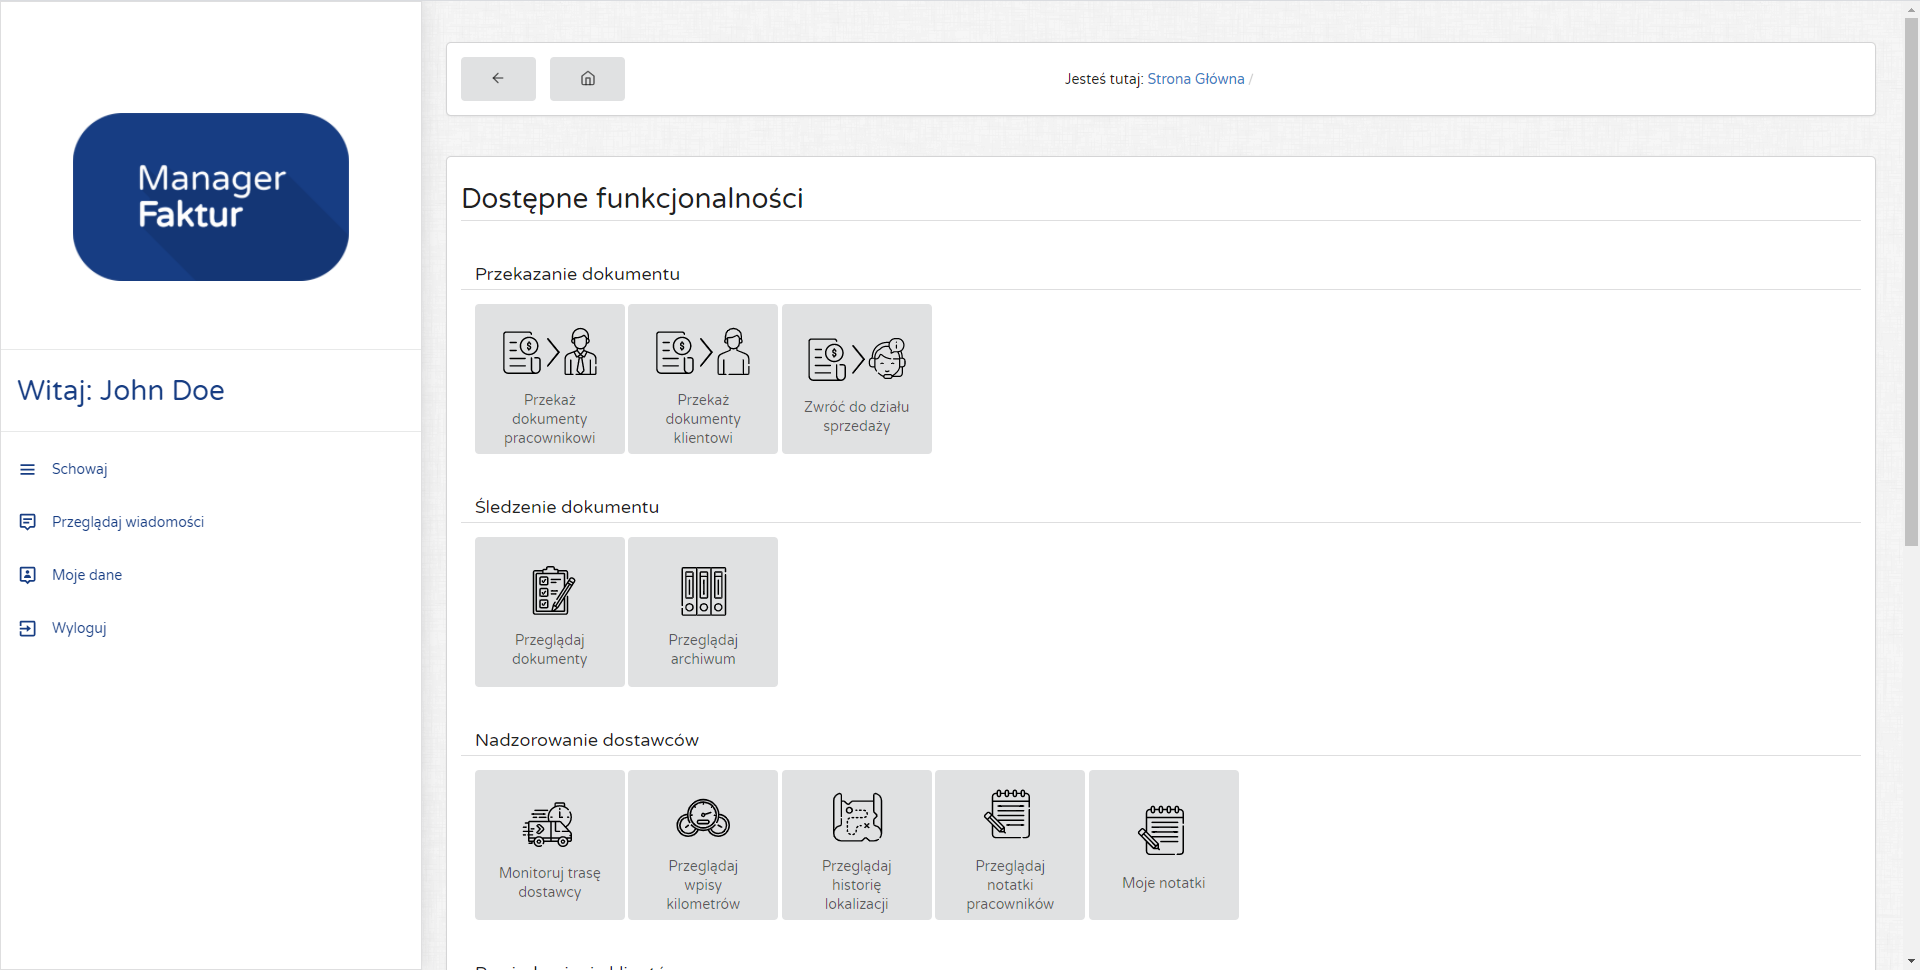
\includegraphics[width=0.95\linewidth]{rys04/zrzut1}
 \caption{Widok panelu głównego aplikacji webowej}
 \label{fig:gui-webowa-zrzut1}
\end{figure}

\begin{figure}[ht]
 \centering
  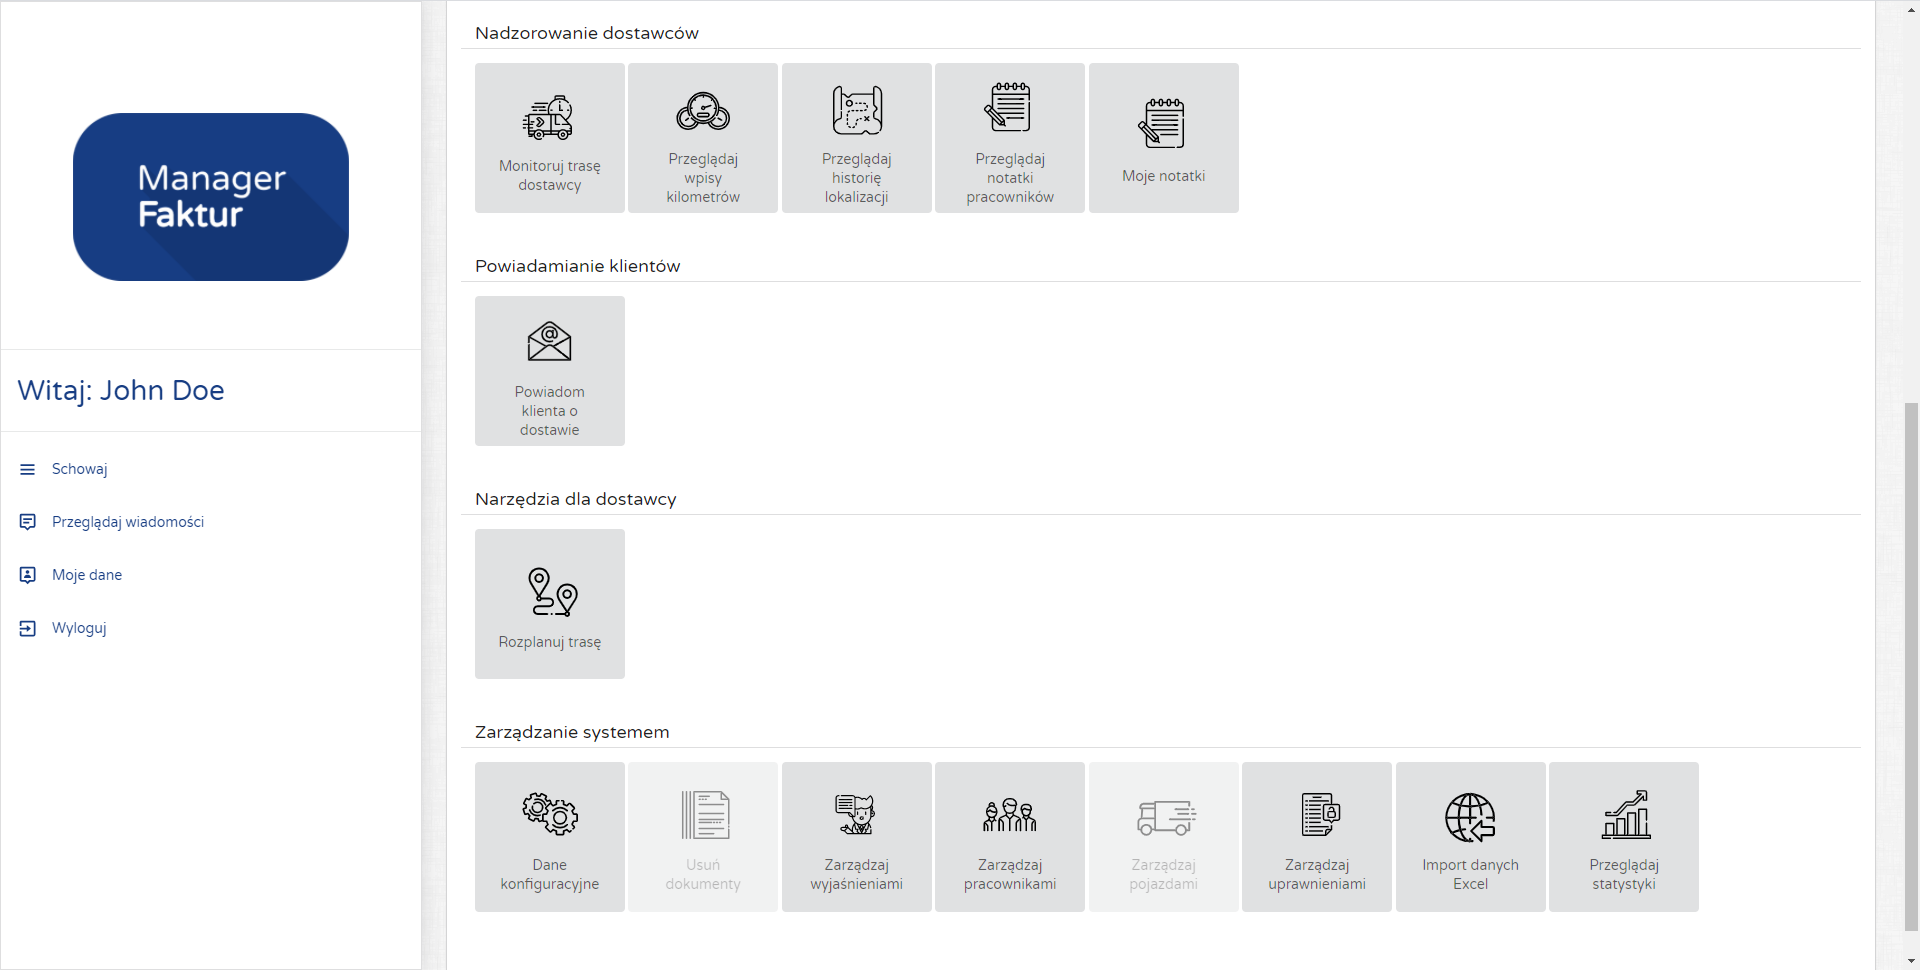
\includegraphics[width=0.95\linewidth]{rys04/zrzut2}
 \caption{Widok panelu głównego aplikacji webowej (cz 2.)}
 \label{fig:gui-webowa-zrzut2}
\end{figure}

Na ilustracjach \ref{fig:gui-webowa-zrzut1} i \ref{fig:gui-webowa-zrzut2} ukazano widok panelu głównego aplikacji webowej. Użytkownik przechodzi z nich do innych widoków, wybierając określony przycisk funkcjonalności. Przyciski widoków mogą być aktywne lub niedostępne, w zależności od posiadanych przez pracownika uprawnień.

\begin{figure}[ht]
 \centering
  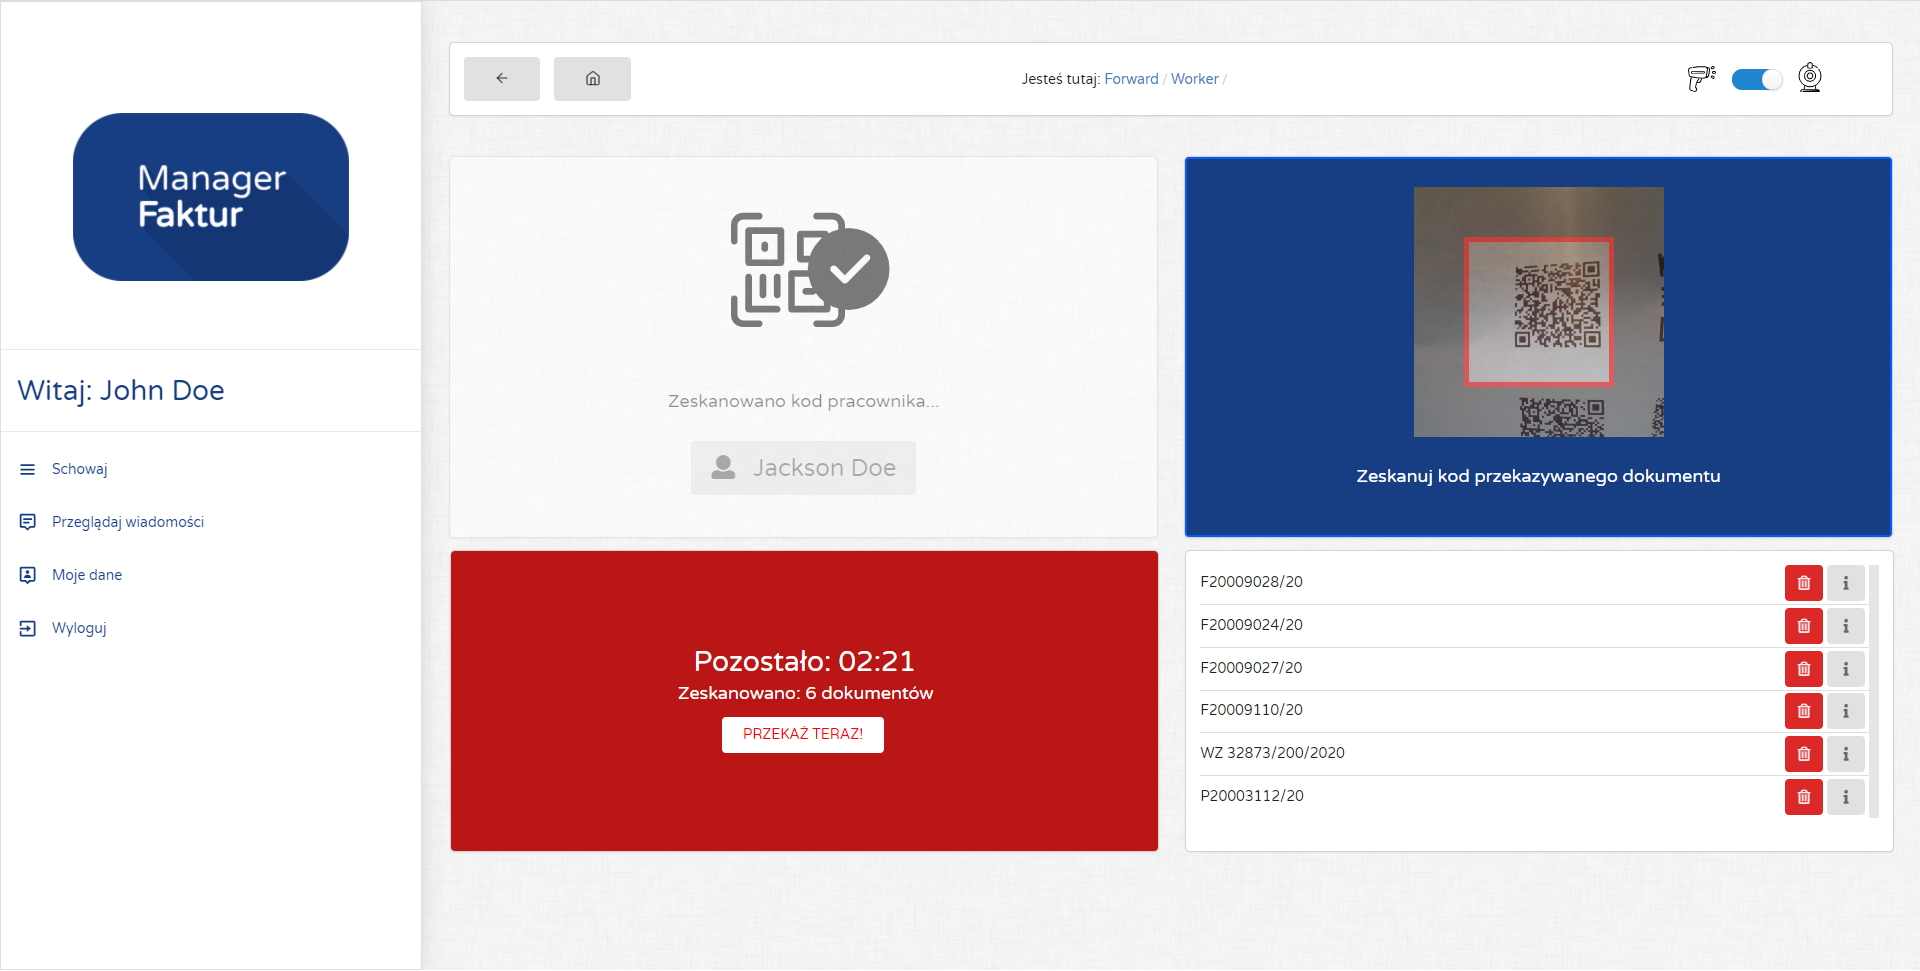
\includegraphics[width=0.95\linewidth]{rys04/zrzut3}
 \caption{Widok funkcjonalności przekazywania dokumentów pracownikowi}
 \label{fig:gui-webowa-zrzut3}
\end{figure}

Na rysunku \ref{fig:gui-webowa-zrzut3} widzimy moduł przekazywania dokumentów pomiędzy pracownikami. W momencie tworzenia tej ilustracji, zeskanowany został kod pracownika, a wczytywany zostaje barkod QR dokumentu. Poniżej widoku kamery, zlokalizowane są dwa kontenery, prezentujące czas pozostały do zakończenia procedury skanowania oraz listę wczytanych dokumentów.

\begin{figure}[ht]
 \centering
  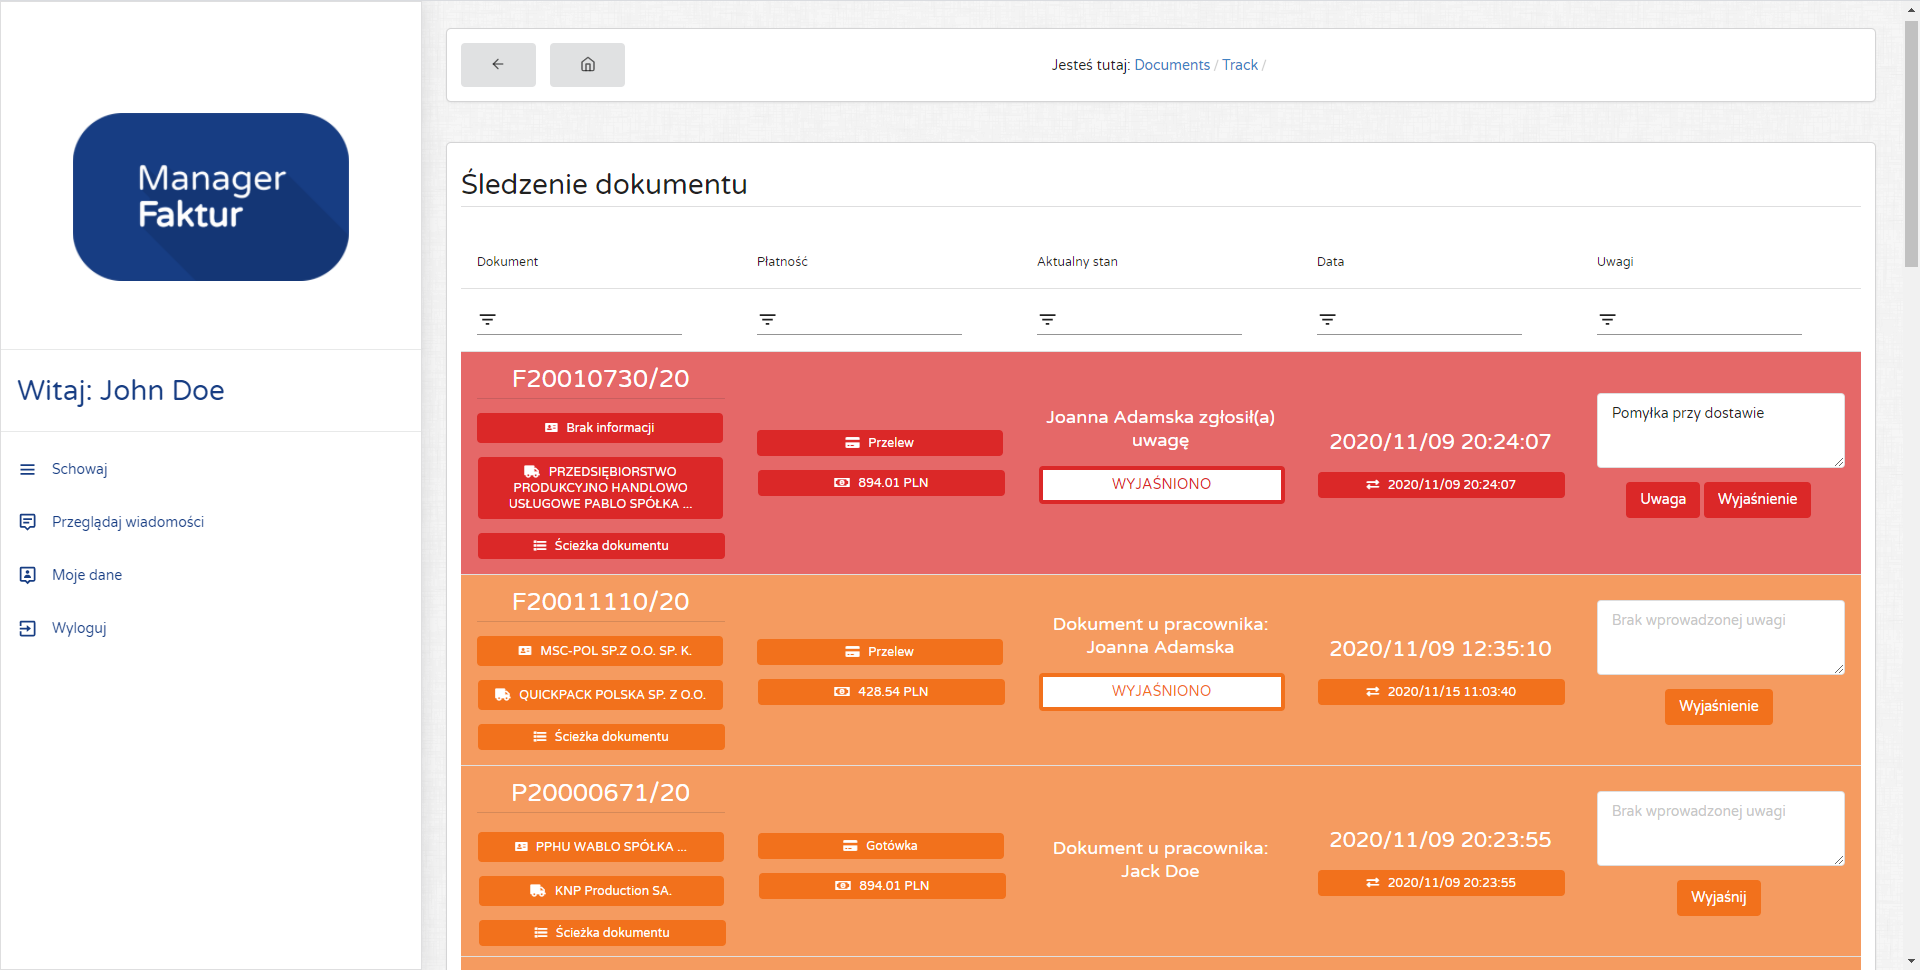
\includegraphics[width=0.95\linewidth]{rys04/zrzut4}
 \caption{Widok funkcjonalności śledzenia dokumentów}
 \label{fig:gui-webowa-zrzut4}
\end{figure}

Ilustracja \ref{fig:gui-webowa-zrzut4} obrazuje widok śledzenia dokumentów. W każdym wierszu tabeli, prezentowane są informacje o dokumencie, jego aktualnym statusie w systemie, a także wszystkich akcjach na nim wykonanych. Użytkownik, posiadający uprawnienia dostępu do tego widoku, może ponadto wprowadzić notę wyjaśniającą dla dokumentu (przycisk "`Wyjaśnij"'), co spowoduje archiwizację faktury po zakończeniu dnia pracy.

\begin{figure}[ht]
 \centering
  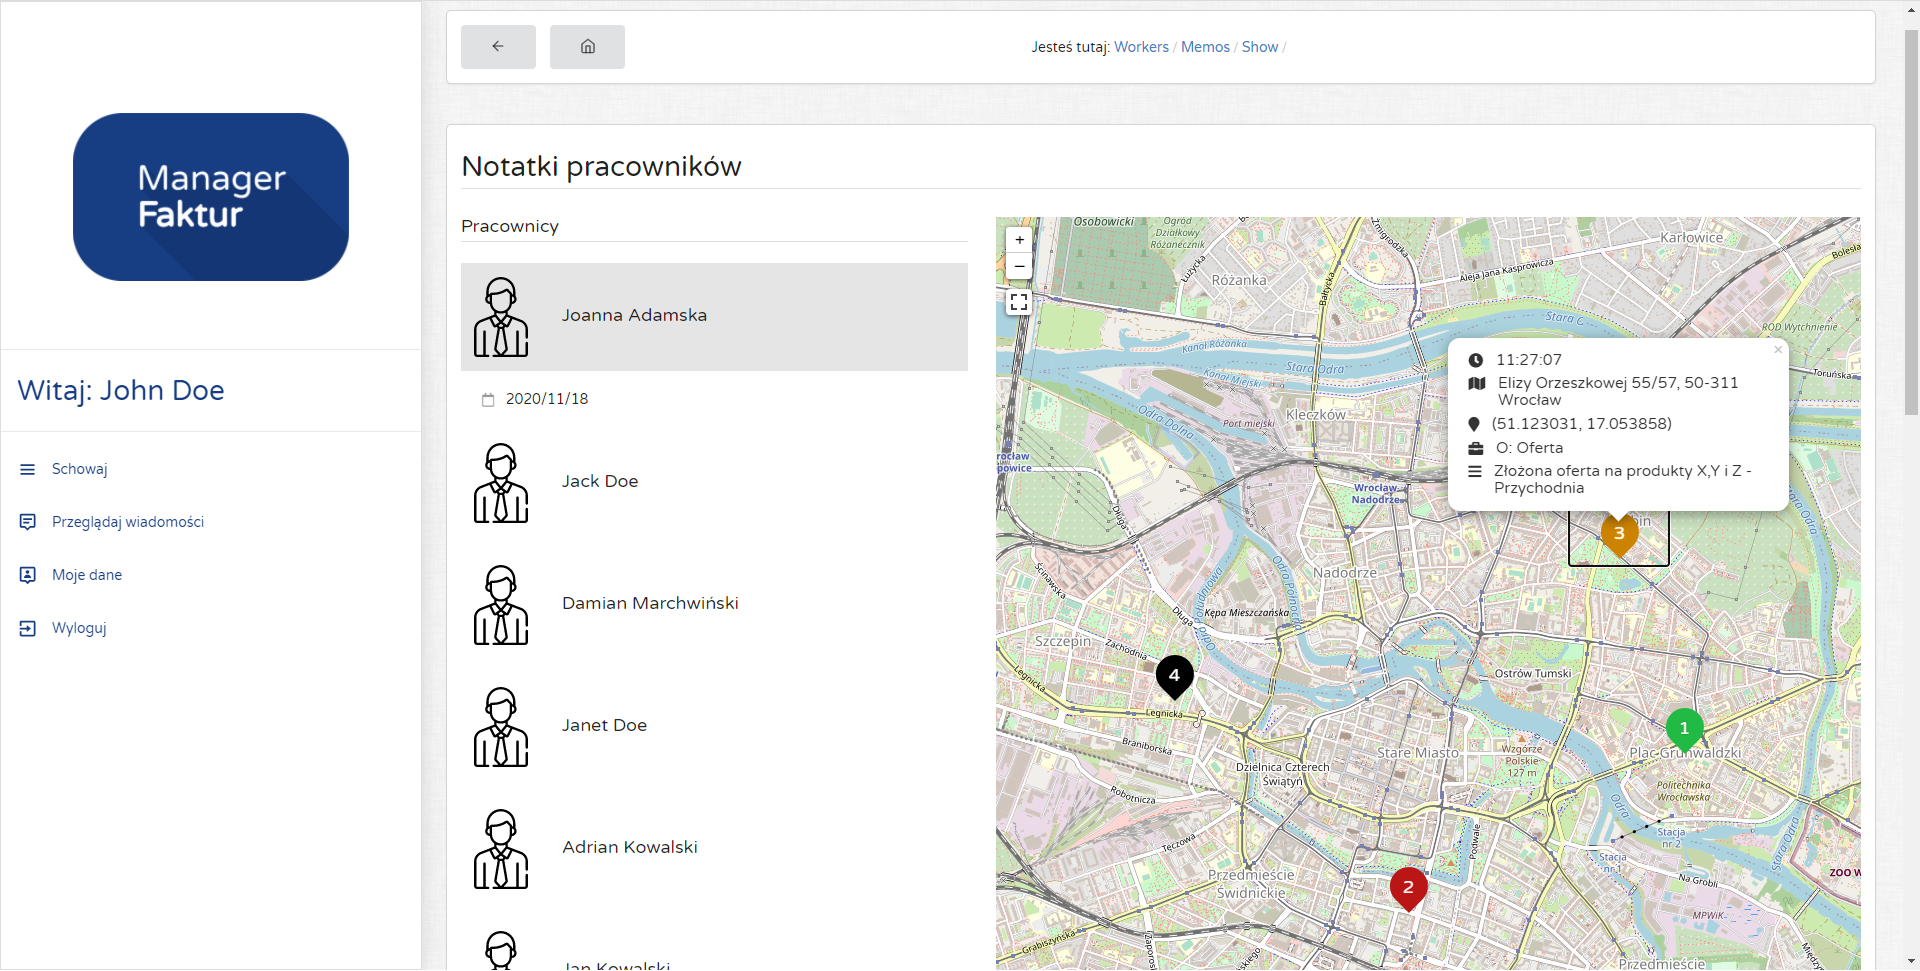
\includegraphics[width=0.95\linewidth]{rys04/zrzut5}
 \caption{Widok funkcjonalności przeglądania notatek pracowników handlowych}
 \label{fig:gui-webowa-zrzut5}
\end{figure}

Przedstawiona grafika \ref{fig:gui-webowa-zrzut5} ukazuje widok modułu przeglądania notatek handlowych. Użytkownik, w ramach tego widoku, po wybraniu pracownika oraz daty utworzenia notatek, może przeglądać wszystkie wprowadzone przez pracownika wpisy informacyjne. W zależności od typu wpisu, ukazane na mapie punkty lokalizacyjne, charakteryzują się odmienną kolorystyką. Po wybraniu określonego punktu na mapie, widoczne są dane notatki dla tej lokalizacji.

\begin{figure}[ht]
 \centering
  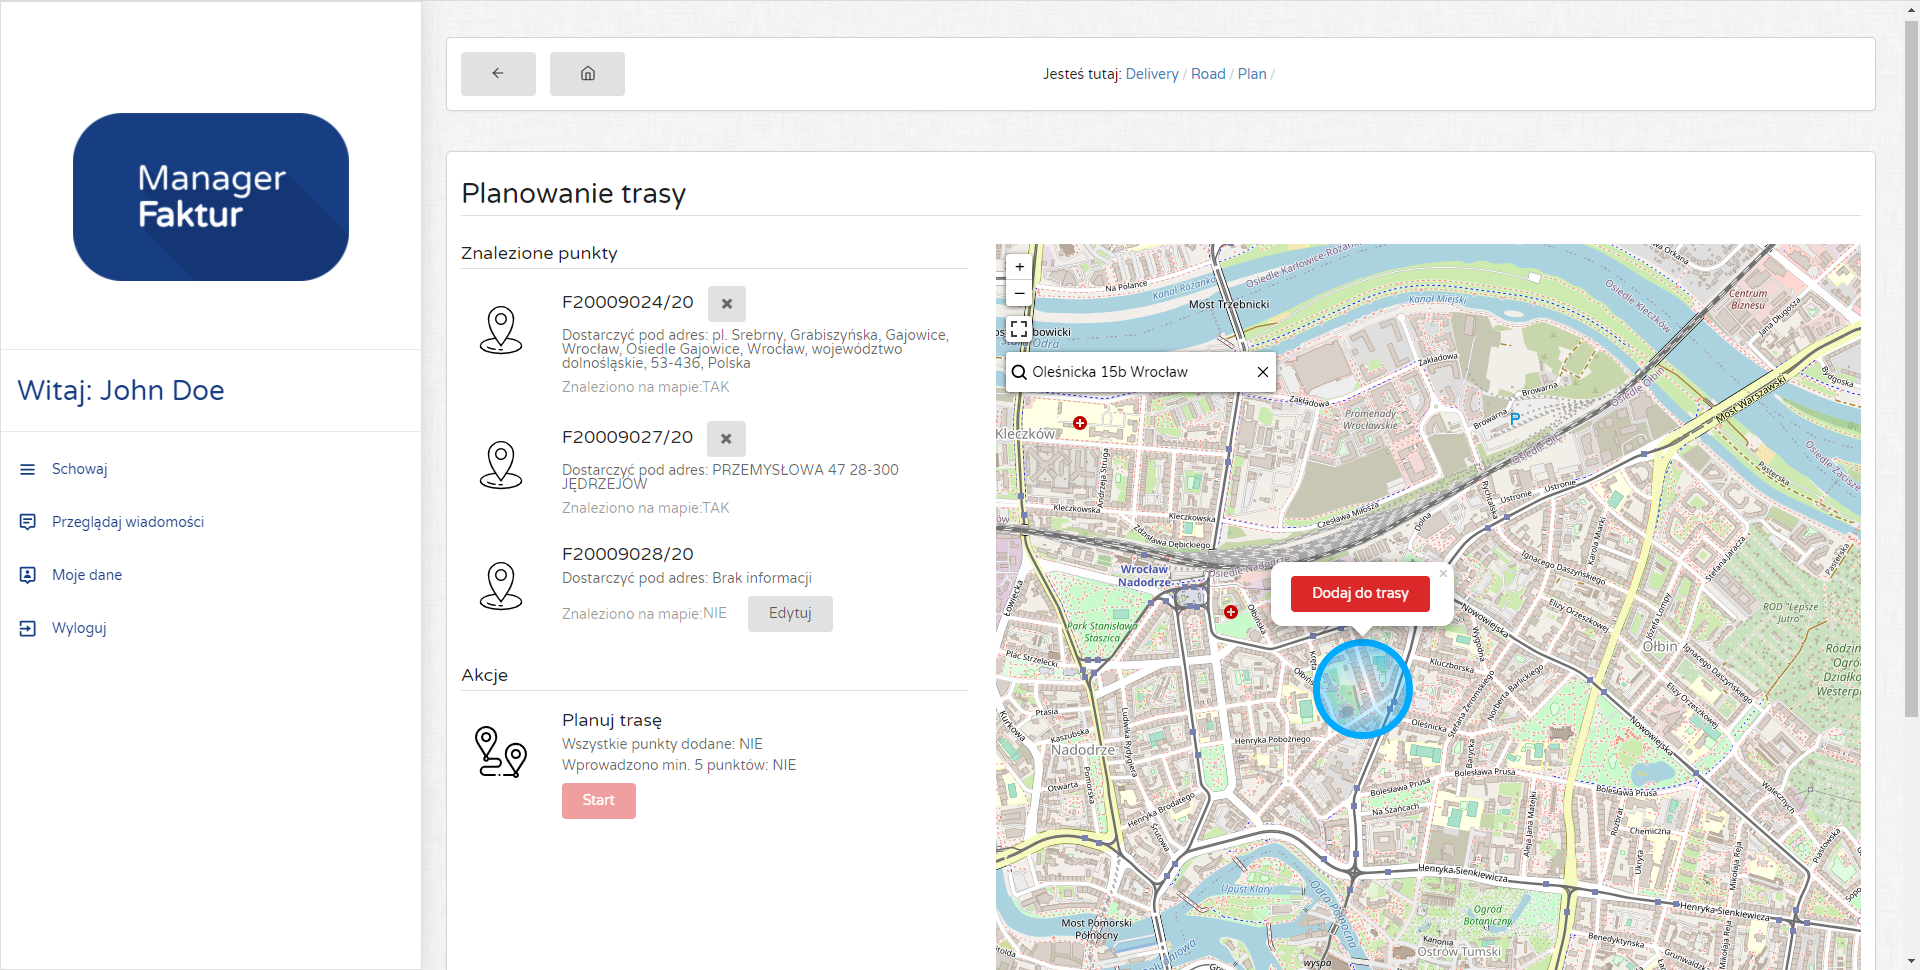
\includegraphics[width=0.95\linewidth]{rys04/zrzut6}
 \caption{Widok funkcjonalności planowania trasy dostawy - wybór lokalizacji}
 \label{fig:gui-webowa-zrzut6}
\end{figure}

Na ilustracji \ref{fig:gui-webowa-zrzut6}, widoczny jest element segmentu planowania trasy dostawy. Po lewej stronie widoku, dostępne są wszystkie dokumenty przypisane do zalogowanego pracownika, natomiast po prawej stronie, znajduje się fragment mapy. Mapa ta, wykorzystywana jest do wyboru lokalizacji dostawy dla dokumentu, w sytuacji gdy dane faktury nie pozwolą na jej automatyczne uzyskanie.

\newpage

\begin{figure}[ht]
 \centering
  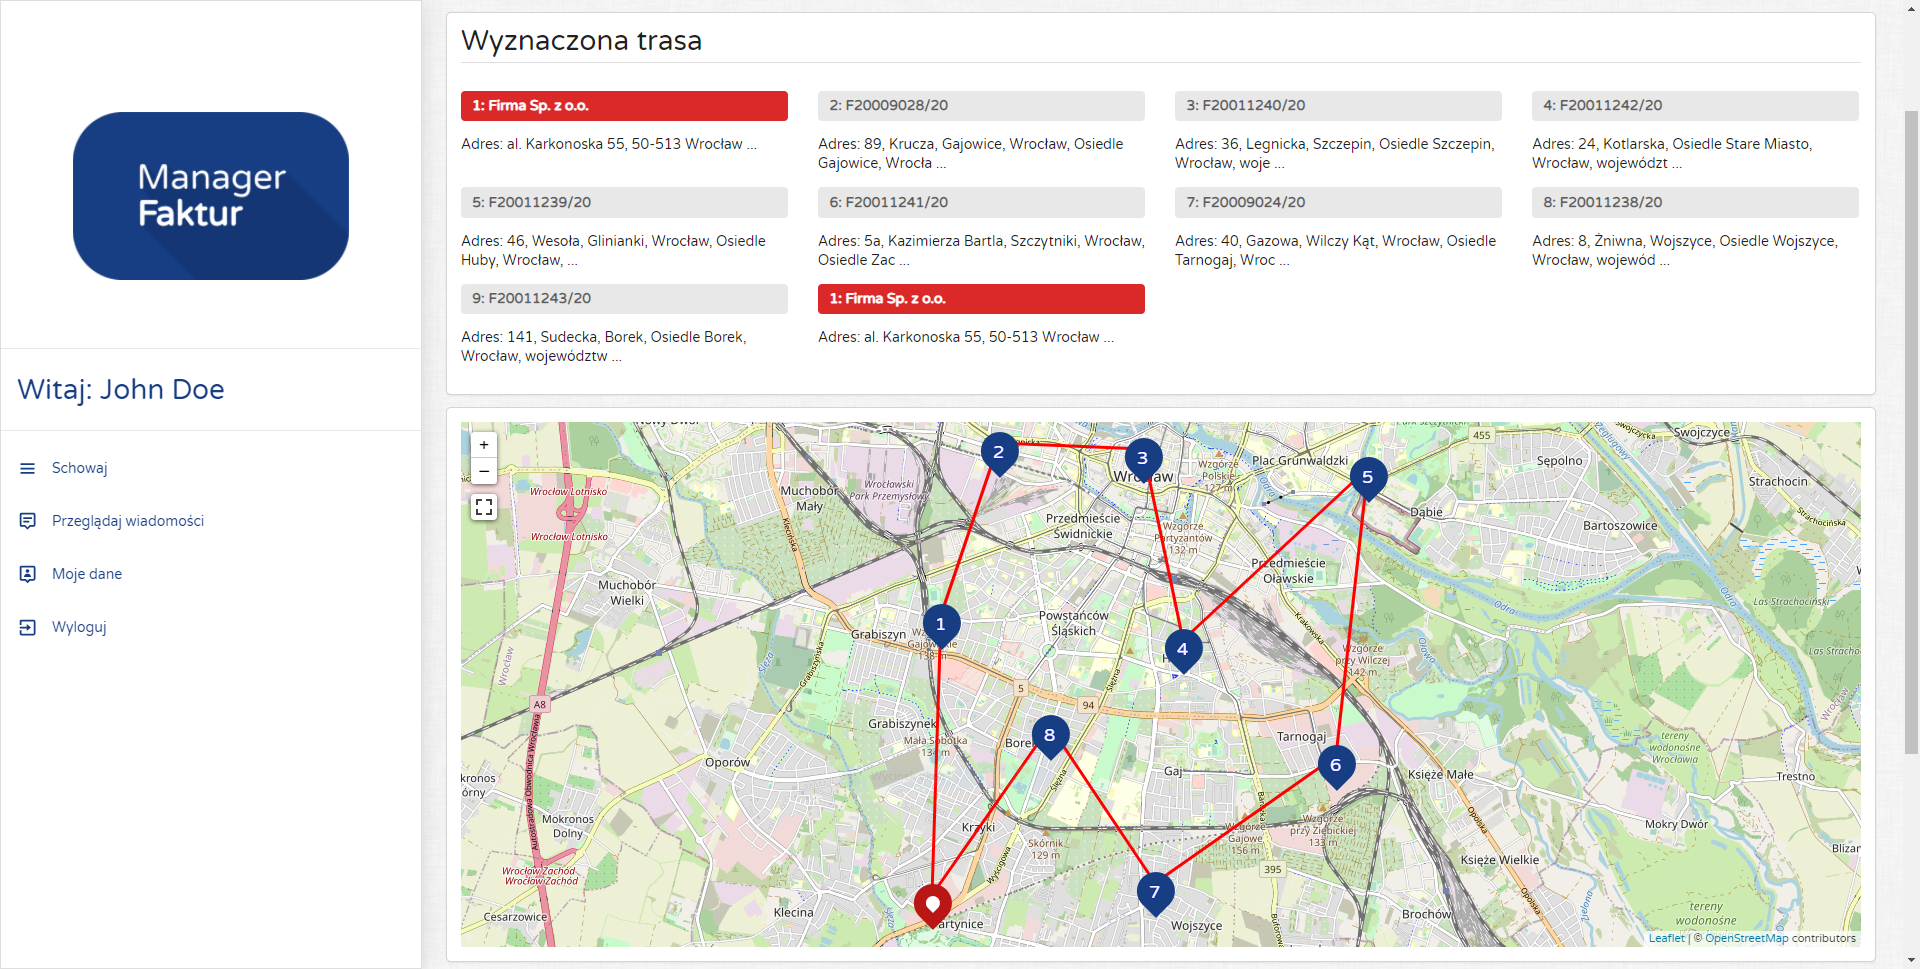
\includegraphics[width=0.95\linewidth]{rys04/zrzut7}
 \caption{Widok funkcjonalności planowania trasy dostawy - rezultat}
 \label{fig:gui-webowa-zrzut7}
\end{figure}

Po wyborze wszystkich punktów lokalizacyjnych, uruchamiany jest algorytm wyliczania trasy dostawy. Z chwilą otrzymania wyniku działania algorytmu, ukazuje się widok przedstawiony na ilustracji \ref{fig:gui-webowa-zrzut7}. Widzimy w nim listę kolejnych lokalizacji na drodze dostawy, a także mapę unaoczniającą sekwencję odwiedzanych punktów. Po wybraniu dowolnego z punktów, wyświetlana jest informacja o powiązanym dokumencie oraz danych adresowych.

\begin{figure}[ht]
 \centering
  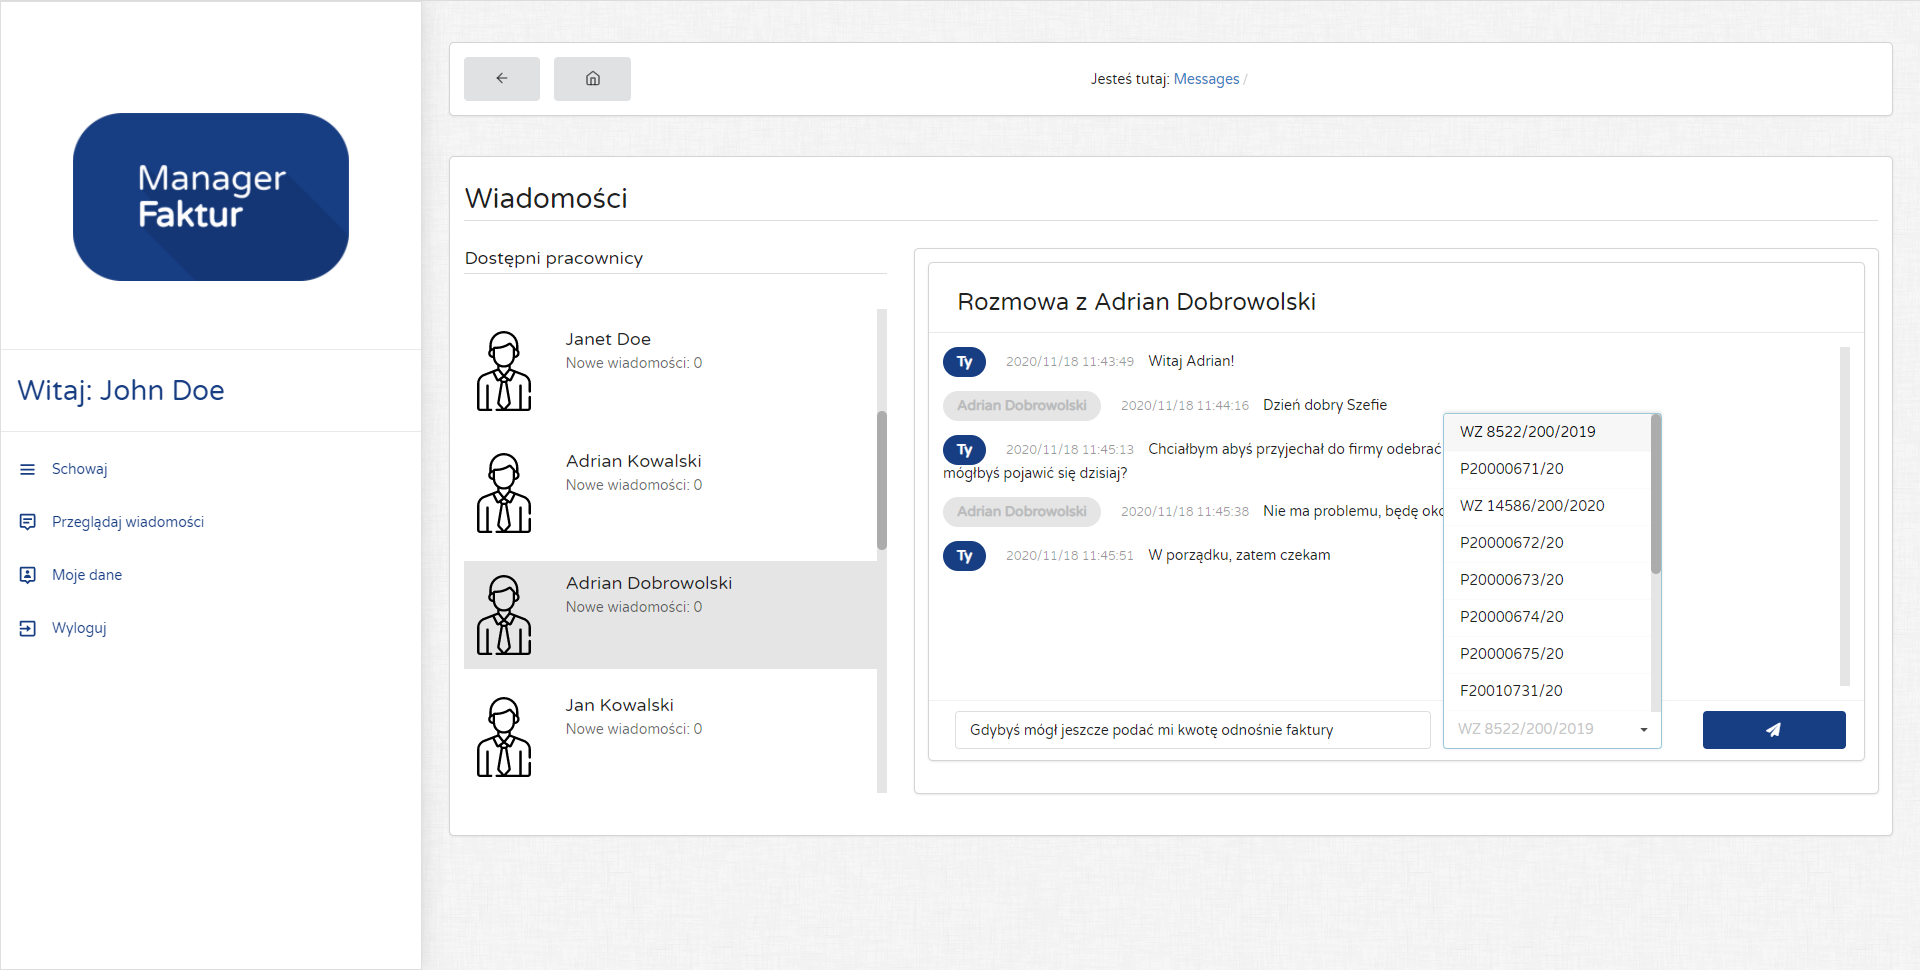
\includegraphics[width=0.95\linewidth]{rys04/zrzut8}
 \caption{Widok funkcjonalności komunikatora tekstowego}
 \label{fig:gui-webowa-zrzut8}
\end{figure}

Rysunek \ref{fig:gui-webowa-zrzut8}, prezentuje wygląd widoku wewnętrznego komunikatora tekstowego. Wyróżnić możemy w nim listę pracowników, z którymi chcemy rozpocząć konwersację, a także okno wysyłanych wiadomości. Poza możliwością wprowadzania tekstu wiadomości, istnieje także funkcjonalność wyboru dokumentu, o którym chcemy "`wspomnieć"' w wiadomości. Wprowadzenie wspomnienia dla faktury, skutkuje wyświetleniem adekwatnej informacji, w widoku śledzenia dokumentów.

\newpage

\begin{figure}[ht]
  \centering
	\begin{tabular}{@{}ll@{}}
	a) & b) \\
  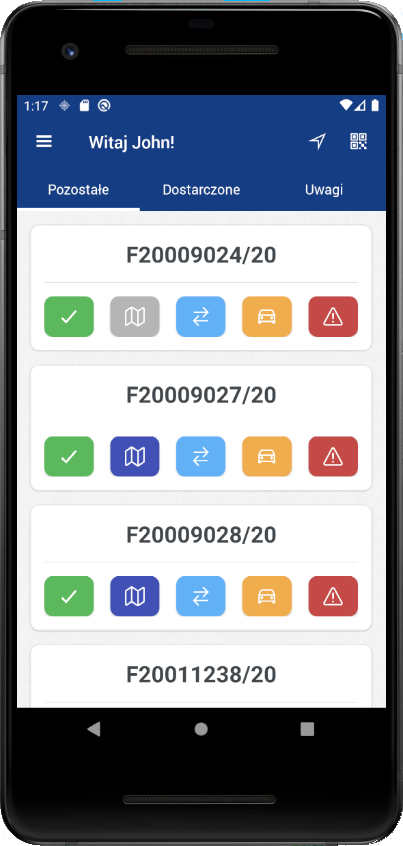
\includegraphics[width=0.3\textwidth]{rys04/mobilna/zrzut1} & 
	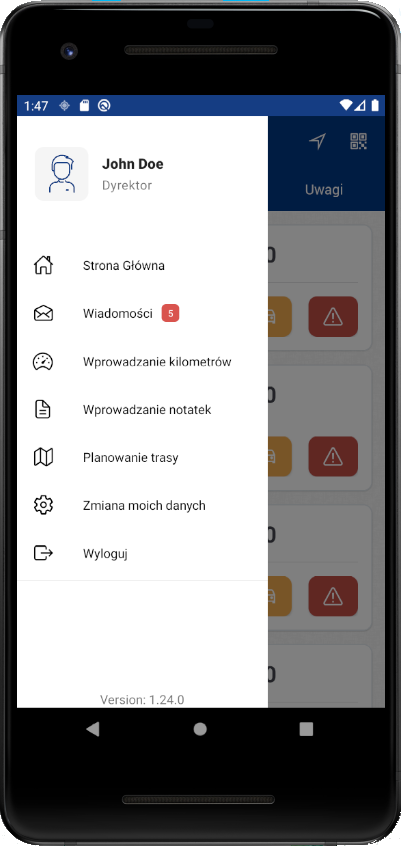
\includegraphics[width=0.3\textwidth]{rys04/mobilna/zrzut2}
	\end{tabular}
  \caption{Aktywność główna aplikacji mobilnej a) lista dokumentów b) panel boczny}
  \label{fig:gui-mobilna-zrzut12}
\end{figure}

Na ilustracjach \ref{fig:gui-mobilna-zrzut12}a oraz \ref{fig:gui-mobilna-zrzut12}b, przedstawiona została aktywność główna aplikacji mobilnej. Pierwsza z grafik, ukazuje widok listy dokumentów, ładowany domyślnie, po zalogowaniu się do systemu. Na drugim rysunku natomiast, widzimy rozsuwany panel boczny, zawierający większość z dostępnych funkcjonalności aplikacji.

\begin{figure}[ht]
  \centering
	\begin{tabular}{l l l}
	a) & b) & c) \\
  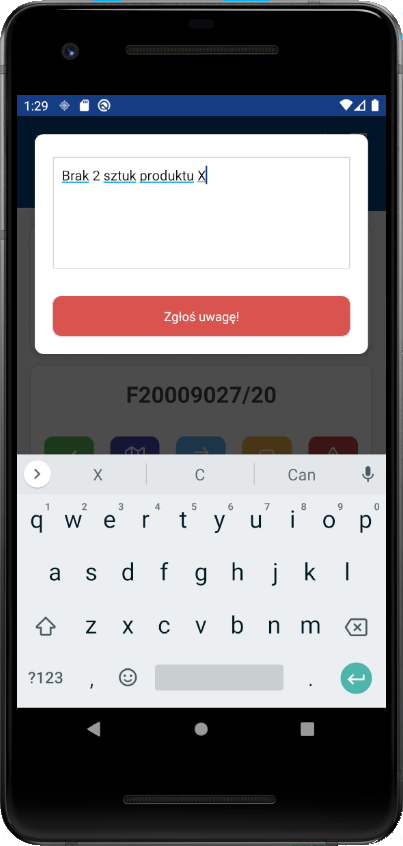
\includegraphics[width=0.27\textwidth]{rys04/mobilna/zrzut3} & 
	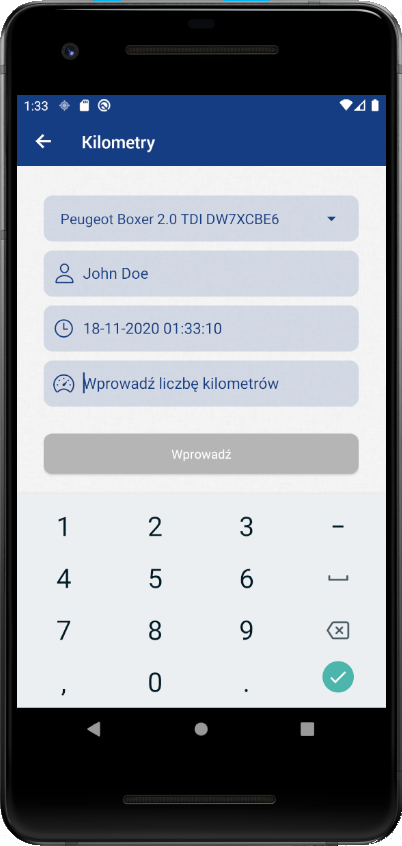
\includegraphics[width=0.27\textwidth]{rys04/mobilna/zrzut4} &
	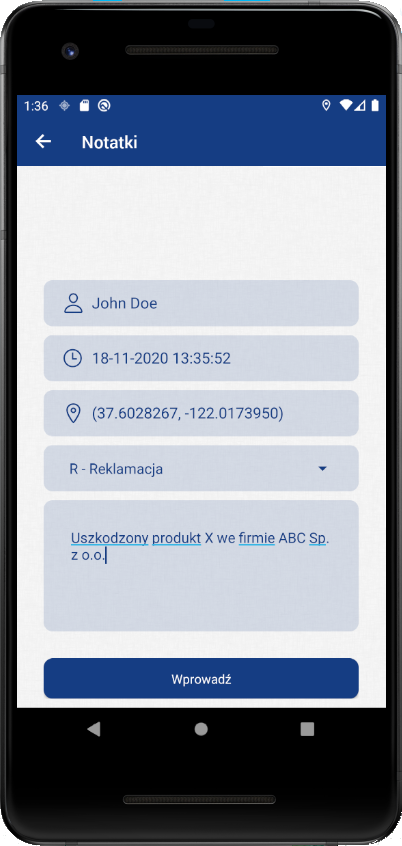
\includegraphics[width=0.27\textwidth]{rys04/mobilna/zrzut5}
	\end{tabular}
  \caption{Aktywności wprowadzania danych a) zgłaszanie uwagi b) wpis kilometrów c) wpis notatki}
  \label{fig:gui-mobilna-zrzut345}
\end{figure}

W ramach rysunków \ref{fig:gui-mobilna-zrzut345}a, \ref{fig:gui-mobilna-zrzut345}b oraz \ref{fig:gui-mobilna-zrzut345}c, ukazane zostały aktywności wprowadzania danych w aplikacji mobilnej. Pierwsza z nich, tyczy się zgłaszania uwagi dotyczącej dokumentu. Użytkownik, po naciśnięciu czerwonego przycisku, znajdującego się przy fakturze, wprowadza zawartość notatki uwagi, do przedstawionego pola tekstowego. Druga aktywność, zdefiniowana została w celu generowania adnotacji dotyczących liczników kilometrów, w pojazdach firmy. W widoku tym, jeżeli do użytkownika przypisany jest pojazd domyślny, zostaje on wybrany z listy rozwijanej automatycznie. Trzecia z aktywności, wykorzystywana jest do wprowadzania wpisów dotyczących notatek handlowych. 

\begin{figure}[ht]
  \centering
	\begin{tabular}{l l l}
	a) & b) & c) \\
  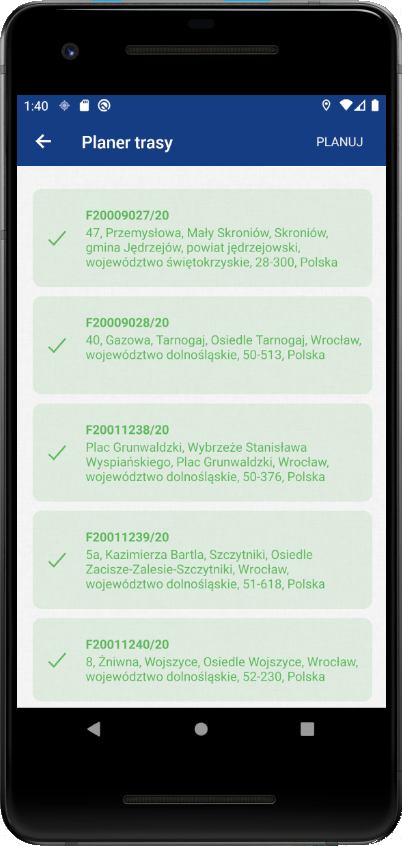
\includegraphics[width=0.27\textwidth]{rys04/mobilna/zrzut6} & 
	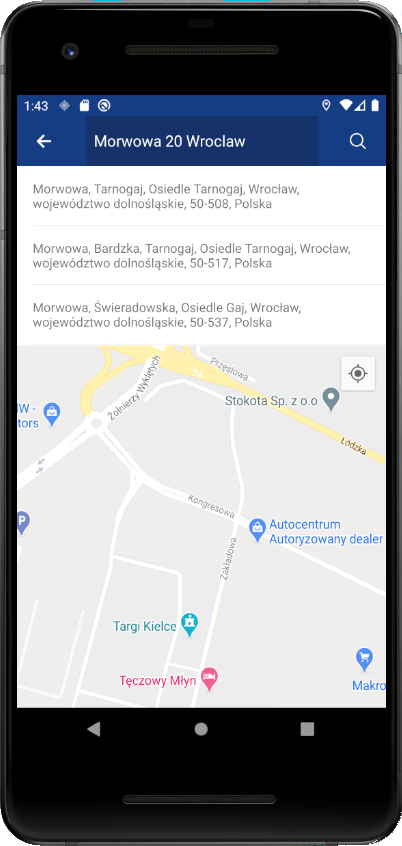
\includegraphics[width=0.27\textwidth]{rys04/mobilna/zrzut8} &
	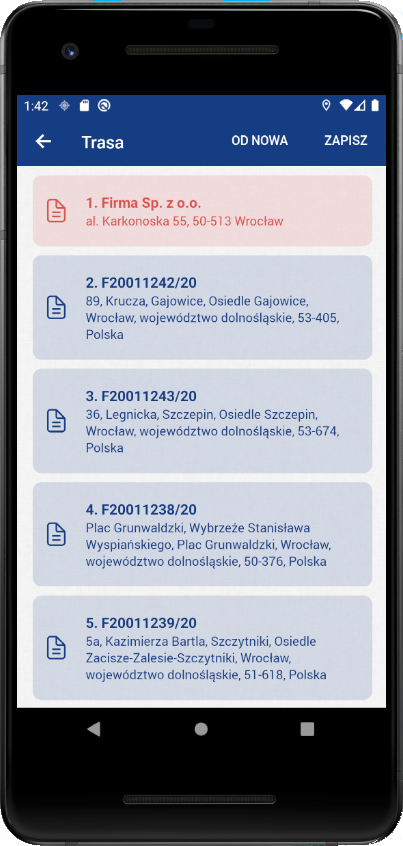
\includegraphics[width=0.27\textwidth]{rys04/mobilna/zrzut7}
	\end{tabular}
  \caption{Aktywności planowania trasy dostawy a) lista dokumentów b) wybór lokalizacji c) rezultat obliczeń}
  \label{fig:gui-mobilna-zrzut678}
\end{figure}

Na grafikach \ref{fig:gui-mobilna-zrzut678}a, \ref{fig:gui-mobilna-zrzut678}b oraz \ref{fig:gui-mobilna-zrzut678}c, widzimy widoki aplikacji mobilnej, dotyczące wyznaczania trasy dostawy. W pierwszym widoku, zawarta jest lista przypisanych do pracownika dokumentów. Po wybraniu jednej z faktur, jeżeli nie posiada ona przypisanej automatycznie lokalizacji, przechodzimy do aktywności drugiej. W ramach tej aktywności, użytkownik może wyszukać dowolną lokalizację, a następnie przypisać ją do dokumentu. Widok trzeci natomiast, reprezentuje rezultat, w postaci ustalonej trasy dostawy. Po kliknięciu przycisku "`zapisz"', użytkownik kierowany jest do panelu głównego, a dokumenty w nim zawarte, sortują się w kolejności zgodnej z trasą dostawy.

\newpage

\begin{figure}[ht]
  \centering
	\begin{tabular}{@{}ll@{}}
	a) & b) \\
  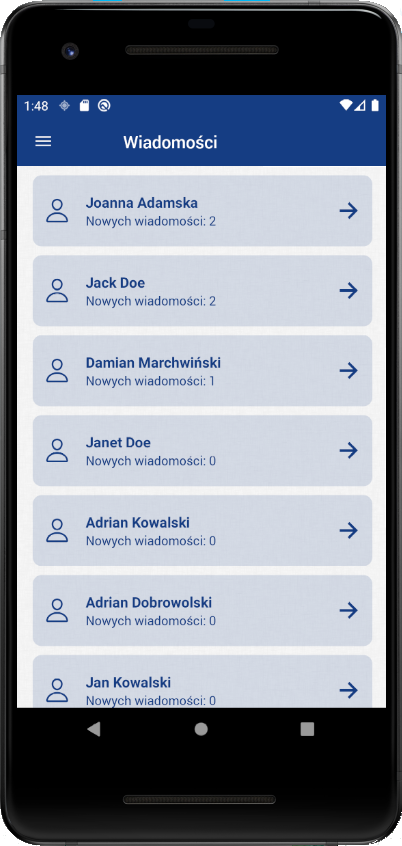
\includegraphics[width=0.3\textwidth]{rys04/mobilna/zrzut9} & 
	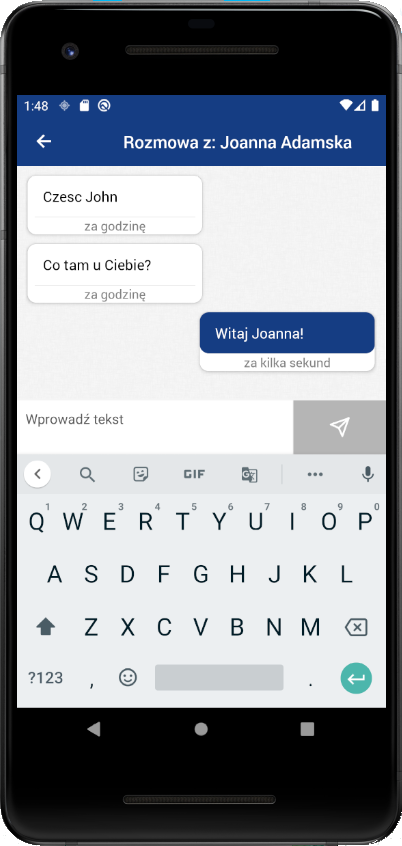
\includegraphics[width=0.3\textwidth]{rys04/mobilna/zrzut10}
	\end{tabular}
  \caption{Aktywność komunikatora aplikacji mobilnej a) lista pracowników b) wymiana wiadomości}
  \label{fig:gui-mobilna-zrzut910}
\end{figure}

Ostatnie z przedstawionych grafik (tj. grafika \ref{fig:gui-mobilna-zrzut910}a oraz \ref{fig:gui-mobilna-zrzut910}b), ukazują funkcjonalność wewnętrznego komunikatora tekstowego aplikacji mobilnej. Wyróżnić możemy tutaj widok listy pracowników, w którymi można rozpocząć konwersację, a także komponent przedstawiający rozmowę z konkretnym użytkownikiem.
